\chapter{Xây dựng phiên bản thử nghiệm}
\section{Công nghệ sử dụng}
Để hiện thực hệ thống, nhóm quyết định sử dụng các công nghệ sau:
\begin{itemize}
    \item ReactJS: Hiện thực UI, frontend.
    \item Java Springboot: Hiện thực microservice, backend.
    \item PostgresSQL: Hệ cơ sở dữ liệu lưu trữ thông tin.
    \item Kubernetes: Deploy các microservice.
    \item Minikube: Chạy Kubernetes cluster trên local.
    \item Terraform: Khởi tạo 
\end{itemize}

\section{Giới hạn phạm vi}
\subsection{Về mặt nghiệp vụ}
\noindent Sau khi bàn bạc, nhóm đi tới thống nhất là sẽ hiện thực phần Trang chủ (Home page - Catalog), vì đó là thành phần mà người dùng sẽ gặp đầu tiên khi bắt đầu truy cập vào hệ thống.
\subsection{Về mặt thành phần hệ thống}
\noindent Sau khi cân nhắc kỹ lưỡng, để đảm bảo cho phiên bản demo thể hiện được trọn vẹn và đầy đủ nhất các tính chất cốt lõi của hệ thống, nhóm đã giới hạn phạm vi hiện thực của hệ thống xuống còn các thành phần như sau:
\begin{itemize}
    \item Frontend: Trang chủ - Catalog, thể hiện danh sách các mặt hàng đang được bày bán 
    \item Backend: Catalog service, cung cấp API danh sách sản phẩm.
    \item Minikube cluster: Cung cấp môi trường Kubernetes cluster local trên máy tính cá nhân.
    \item Deployment: Thành phần cơ bản nhất của hệ thống, dùng để quản lý trực tiếp các pod.
    \item Service: Một lớp ảo hóa để các thành phần khác có thể truy cập tới các pod.
    \item Ingress: Đóng vai trò như reverse proxy, cung cấp API gateway để kết nối từ bên ngoài cluster tới service.
    \item Horizontal Pod Autoscaler: Dùng để tăng hoặc giảm số pod một cách tự động, dựa trên các thông số (metrics) của chính các pod đó.
\end{itemize}
\section{Nội dung hiện thực}
\subsection{Hiện thực frontend và backend}
\noindent Sau khi có một ứng dụng hoàn chỉnh, có thể hiển thị được thông tin mặt hàng, ta đóng gói nó thành Docker image và đẩy lên Docker Hub.\\[0.5cm]
Dockerfile của frontend có nội dung như sau:
\begin{lstlisting}[language=docker]
# Use an official Node runtime as a parent image
FROM node:18 AS builder

# Set the working directory in the container
WORKDIR /app

# Copy package.json and package-lock.json to the container
COPY package.json ./

# Install dependencies
RUN npm install

# Copy the rest of the application code to the container
COPY . .

# Build the Vite React application
RUN npm run build

# Use an official Nginx runtime as a parent image
FROM nginx:alpine

# Copy the build output from the builder stage to the nginx web root
COPY --from=builder /app/dist /usr/share/nginx/html

# Expose port 80
EXPOSE 80
\end{lstlisting}

Dockerfile của backend có nội dung như sau:

\begin{lstlisting}[language=docker]
# Use an official OpenJDK runtime as a base image with Java 17
FROM eclipse-temurin:17-jdk-alpine

# Set the working directory to /app
WORKDIR /app

# Copy the current directory contents into the container at /app
COPY . /app

# Build the Spring Boot application
RUN ./mvnw package -DskipTests

# Expose the port that your Spring Boot application will run on
EXPOSE 80

# Define the command to run your application
CMD ["java", "-jar", "target/catalog-0.0.1-SNAPSHOT.jar"]
\end{lstlisting}

\subsection{Hiện thực Deployment và Service}
\noindent Ta sử dụng terraform để khởi tạo các service trên, tương ứng với mỗi microservice frontend và backend.
\subsubsection{Với frontend}
\noindent Với frontend, khi được đưa lên production, service sẽ được build thành định dạng html, css truyền thống, đi kèm với file javascript chứa logic, và được cung cấp bởi Nginx server, do đó mặc định port sẽ là 80 (HTTP).
\begin{lstlisting}[language=terraform]
resource "kubernetes_deployment" "catalog-fe-deploy" {
  metadata {
    name = "catalog-fe-deploy"
    labels = { app = "catalog-fe", tier = "frontend" }
  }
  spec {
    replicas = 1
    selector {
      match_labels = { app = "catalog-fe-pod", tier = "frontend" }
    }
    template {
      metadata {
        name = "catalog-fe-pod"
        labels = { app = "catalog-fe-pod", tier = "frontend"}
      }
      spec {
        container {
          name = "catalog-fe"
          image = "hoanganhleboy/catalog-fe:latest"
          port { container_port = 80 }
          env {
            name = "CONTENT"
            value = "This is the string from k8s"
          }
          image_pull_policy = "Always"
        }
      }
    }
  }
}

resource "kubernetes_service" "catalog-fe-service" {
  metadata {
    name = "catalog-fe-service"
    labels = { app = "catalog-fe-service", tier = "frontend" }
  }
  spec {
    selector = { app = "catalog-fe-pod", tier = "frontend"}
    port {
      protocol = "TCP"
      port = 80
      target_port = 80
    }
    type = "NodePort"
  }
}
\end{lstlisting} 
\subsubsection{Với backend}
\noindent Catalog microservice sau khi được build thành image sẽ được chạy từ file .jar, thông qua JVM.
\begin{lstlisting}[language=terraform]
resource "kubernetes_deployment" "catalog-ms-deploy" {
  metadata {
    name = "catalog-ms-deploy"
    labels = { app = "catalog-ms", tier = "backend" }
  }
  spec {
    replicas = 1
    selector {
      match_labels = { app = "catalog-ms-pod", tier = "backend" }
    }
    template {
      metadata {
        name = "catalog-ms-pod"
        labels = { app = "catalog-ms-pod", tier = "backend"}
      }
      spec {
        container {
          name = "catalog-ms"
          image = "hoanganhleboy/catalog-ms"
          port { container_port = 8090 } // This port the same with port in the code.
          resources {
            requests = {
              cpu = "256m"
              memory = "128Mi"
            }
            limits = {
              cpu = "256m"
              memory = "128Mi"
            }
          }
        }
      }
    }
  }
}

resource "kubernetes_service" "catalog-ms-service" {
  metadata {
    name = "catalog-ms-service"
    labels = { app = "catalog-ms-service", tier = "backend" }
  }
  spec {
    selector = { app = "catalog-ms-pod", tier = "backend"}
    port {
      protocol = "TCP"
      port = 8090 // port expose to outside
      target_port = 80 // This port the same with port in the code.
    }
    type = "NodePort"
  }
}
\end{lstlisting}
\subsection{Hiện thực Ingress}
\noindent Ingress hiện tại đóng vai trò là reverse proxy, expose các Kubernetes service ra bên ngoài cluster.
\begin{lstlisting}[language=yaml]
apiVersion: networking.k8s.io/v1
kind: Ingress
metadata:
  name: example-ingress
  annotations:
    nginx.ingress.kubernetes.io/enable-directory-listing: "true"
    nginx.ingress.kubernetes.io/rewrite-target: /$2
spec:
  rules:
    - http:
        paths:
          - pathType: Prefix
            path: /backend(/|$)(.*)
            backend:
              service:
                name: catalog-ms-service
                port:
                  number: 80
          - pathType: Prefix
            path: /frontend/?(.*)
            # path: /
            backend:
              service:
                name: catalog-fe-service
                port:
                  number: 80
---

\end{lstlisting}
\subsection{Hiện thực Horizontal Pod Autoscaler}
\noindent Horizontal Pod Autoscaler (HPA) được sử dụng để giúp deployment có thể scale lên và scale xuống số lượng pod tùy theo thông số nào đó của hệ thống. HPA được hiện thực như sau:
\begin{lstlisting}[language=yaml]
apiVersion: autoscaling/v2
kind: HorizontalPodAutoscaler
metadata:
  name: catalog-ms-hpa
spec:
  maxReplicas: 10
  metrics:
  - resource:
      name: cpu
      target:
        averageUtilization: 10
        type: Utilization
    type: Resource
  minReplicas: 1
  scaleTargetRef:
    apiVersion: apps/v1
    kind: Deployment
    name: catalog-ms-deploy
  behavior:
    scaleUp:
      selectPolicy: Max
      stabilizationWindowSeconds: 60
      policies:
      # number of pods that scale in a period of time
        - periodSeconds: 30
          type: Pods
          value: 4
    scaleDown:
      selectPolicy: Min
      stabilizationWindowSeconds: 60
      policies:
      # number of pods that scale in a period of time
        - periodSeconds: 30
          type: Pods
          value: 4
\end{lstlisting}
\section{Kiểm thử hệ thống}
\subsection{Thiết lập}
\noindent Sử dụng minikube, ta tạo một cluster với driver là docker (chạy trên nền docker), bằng câu lệnh \lstinline|minikube start --driver=docker|. Sau đó, ta cần kích hoạt 2 add on cần thiết cho ingress và HPA bằng 2 câu lệnh sau:
\begin{itemize}
  \item \lstinline|minikube addons enable ingress|
  \item \lstinline|minikube addons enable metrics-server|
\end{itemize}
Với addon ingress, ta có thể thiết lập và cấu hình ingress cho cluster. Addon metrics-server đóng vai trò cung cấp, theo dõi các thông số của pod (cpu, memory) nhằm phục vụ cho HPA.\\[0.5cm]
Sau đó, ta sẽ chạy cặp lệnh \lstinline|terraform init| để terraform tải và thiết lập sẵn các dependency cần thiết, và \lstinline|terraform apply --auto-approve| để khởi tạo các dịch vụ Kubernetes được viết bằng terraform.\\[0.5cm]
Với các dịch vụ được viết bằng yaml, ta cần chạy lệnh \lstinline|kubectl apply -f <file_name>| với \lstinline|<file_name>| là tên file config được viết bằng yaml.
\subsection{Kiểm tra tính sẵn sàng - availability}
\noindent Để kiếm tra tính sẵn sàng của hệ thống, ta sẽ thử xóa pod đi xem chuyện gì sẽ xảy ra.\\[0.5cm]
Đây là trạng thái ban đầu của các pod:
\begin{figure}[H]
  \begin{center}
  \includegraphics[scale=0.45]{images/hanh/pod_before_delete.png}
  \caption{Hình ảnh trước khi xóa pod}
  \end{center}
\end{figure}
Còn đây là hình ảnh sau khi vừa xóa:
\begin{figure}[H]
  \begin{center}
  \includegraphics[scale=0.45]{images/hanh/pod_after_delete.png}
  \caption{Hình ảnh sau khi vừa xóa pod}
  \end{center}
\end{figure}
Như ta nhìn thấy trong hình 5.1 và 5.2, khi một pod vừa bị xóa, ngay lập tức một pod khác được khởi động ngay lập tức, thế chỗ cho pod vừa bị xóa. Như vậy, ta có thể kết luận rằng, khi triển khai hệ thống bằng Kubernetes, cụ thể là Deployment, tính sẵn sàng - availability của hệ thống được đảm bảo.
\subsection{Kiếm tra tính mở rộng - scalability}
\subsubsection{Manual scaling}
\noindent Tính mở rộng là việc hệ thống có thể tạo ra thêm nhiều bản sao của microservice, chạy song song với nhau nhằm đáp ứng được lượng request trên giây tương ứng của người dùng. Với Kubernetes, ta có thể dễ dàng scale up hay scale down hệ thống bằng tay thông qua việc điều chỉnh miền \lstinline|replicas| trong file config của Deployment.\\[0.5cm]
Ví dụ như hình 5.3 dưới đây, khi ta tăng số lượng pod của catalog-ms từ 1 lên 3
\begin{figure}[H]
  \begin{center}
    \includegraphics[scale=0.45]{images/hanh/catalog_ms_scale_up.png}
    \caption{Hình ảnh khi scale số pod từ 1 lên 3}
  \end{center}
\end{figure}
Ngay lập tức đã có thêm 2 pod mới được tạo ra như hình. Sau đó, khi ta giảm xuống 1 lại thì:
\begin{figure}[H]
  \begin{center}
    \includegraphics[scale=0.45]{images/hanh/catalog_ms_scale_down.png}
    \caption{Hình ảnh khi scale số pod từ 3 xuống 1}
  \end{center}
\end{figure}
Như hình 5.4, ta thấy ngay lập tức có 2 pod bị xóa đi để đảm bảo số lượng pod trong cluster về đúng số lượng quy định.

\subsubsection{Auto scaling}
Tuy nhiên, trên thực tế, việc scale thủ công như trên sẽ gây tiêu tốn tài nguyên về cả nhân lực và vật lực kha khá, do cần phải có sự can thiệp trực tiếp của con người, và cũng cần con người giám sát 24/24 để đảm bảo có thể điều chỉnh lượng pod phù hợp với nhu cầu lúc đó. Do đó, tốt hơn hết là ta nên thiết lập để Kubernetes có thể thực hiện việc đó một cách tự động thay cho chúng ta, và đó là khi ta cần dùng tới HPA - Horizontal Pod Autoscaler.\\[0.5cm]
Bài kiểm tra bao gồm các bước sau:
\begin{enumerate}
  \item Triển khai Deployment, Service, và HPA cho đối tượng muốn kiểm tra, ở đây là Catalog backend microservice.
  \item Khởi tạo một pod có chứa container được chạy từ image busybox, pod này sẽ cung cấp cho chúng ta môi trường linux shell. Ta sau đó viết 1 đoạn script tạo một vòng lặp vô hạn gọi tới API của Catalog backend microservice.
  \item Sử dụng câu lệnh \lstinline|kubectl get hpa --watch| để theo dõi trạng thái của HPA. Một thời gian sau, khi lượng pod đã được scale tới tối đa, ta tắt script để ngưng gọi API. 
  \item Lại đợi một khoảng thời gian, số pod đã được scale về mức tối thiểu. 
\end{enumerate}
\begin{figure}[H]
  \begin{center}
    \includegraphics[scale=0.19]{images/hanh/HPA_CPU_scale.png}
    \caption{Kết quả cuộc thử nghiệm}
  \end{center}
\end{figure}
\noindent \textbf{Mô tả thí nghiệm:} Trong hình 5.5, ta có thể thấy khi bắt đầu gọi API liên tục tới Catalog backend server, thì CPU load bắt đầu tăng mạnh. Khi CPU load vượt ngưỡng 10\% thì HPA sẽ được kích hoạt để tăng số pod trong deployment lên, nhằm mục đích làm giảm PCU load xuống. Tuy nhiên, một thời gian ngắn sau vì CPU load tiếp tục vượt ngưỡng nên HPA lại tiếp tục được kích hoạt tiếp để tăng thêm số pod ở deployment. Việc này chỉ dừng lại cho đến khi số pod đã đạt ngưỡng tối đa cho phép, hoặc CPU load ổn định không tiếp tục vượt ngưỡng nữa thì thôi.\\[0.5cm]
Sau khi đã scale số pod lên đến mức tối đa là 10, ta terminate busybox đi để ngừng việc gửi request tới Catalog microservice. Lúc này CPU load giảm mạnh xuống còn 0\%. Sau một khoảng thời gian, HPA lại được kích hoạt để giảm số pod xuống. Khi giảm pod, nhận thấy CPU load vẫn tiếp tục dưới ngưỡng, HPA tiếp tục được kích hoạt để giảm tiếp số pod xuống, đến khi nào CPU load xấp xỉ với ngưỡng, hoặc khi đạt đến số pod tối thiểu, ở đây là 1 pod.

\section{Xây dựng tính năng autoscaling với custom metrics (các thông số tùy chỉnh)}
% Tham khảo chính từ 2 bài viết: https://dev.to/k6/how-to-autoscale-kubernetes-pods-with-keda-testing-with-k6-4nl9\influx-grafana và https://devopscube.com/setup-prometheus-monitoring-on-kubernetes/

\subsection{Định nghĩa}
\noindent Theo Google Cloud Platform\footnote{Dựa theo link: https://cloud.google.com/kubernetes-engine/docs/concepts/custom-and-external-metrics}, một \textit{custom metric} sẽ được truyền từ ứng dụng của bạn mà đang chạy trên Kubernetes.
\subsection{Đặt vấn đề}
\noindent Việc scale theo CPU và memory không hiệu quả với rest api.\\
\noindent Mặc dù các số liệu mặc định do Kubernetes cung cấp, chẳng hạn như mức sử dụng CPU và bộ nhớ dựa trên yêu cầu tài nguyên, rất hữu ích trong nhiều tình huống nhưng chúng có thể không đủ cho tất cả các ứng dụng. Mở rộng quy mô dựa trên giới hạn tài nguyên đảm bảo rằng ứng dụng của chúng ta có thể xử lý các khối lượng công việc khác nhau mà không đạt đến mức tài nguyên tối đa được phép. Số liệu tùy chỉnh cho phép chúng ta điều chỉnh hành vi mở rộng quy mô của HPA dựa trên nhu cầu cụ thể của ứng dụng, cho phép tự động điều chỉnh quy mô chính xác và hiệu quả hơn.
\subsection{Cơ sở lý thuyết}
\textit{Nội dung tiểu mục được tham khảo từ chung một nguồn}\footnote{https://learnk8s.io/autoscaling-apps-kubernetes}\\[0.5cm]
% \noindent Nói về việc prometheus dùng để thu thập và cung cấp api server cho external metrics. KEDA cung cấp ScaledObject, được build dựa trên HPA để phục vụ cho việc scale dựa trên các metric thu thập từ prometheus.\\
% \noindent Có thể để các tóm tắt bài viết vào đây.
Khi xác định tài nguyên cho Horizontal Pod Autoscaler, chúng ta cần phải xác định metric mà ta cần theo dõi.

% Nhưng làm cách nào Bộ chia tỷ lệ tự động của Horizontal Pod biết cách lấy được các số liệu này?

Horizontal Pod Autoscaler truy vấn các metrics này từ Metrics Registry.
\begin{figure}[H]
  \begin{center}
    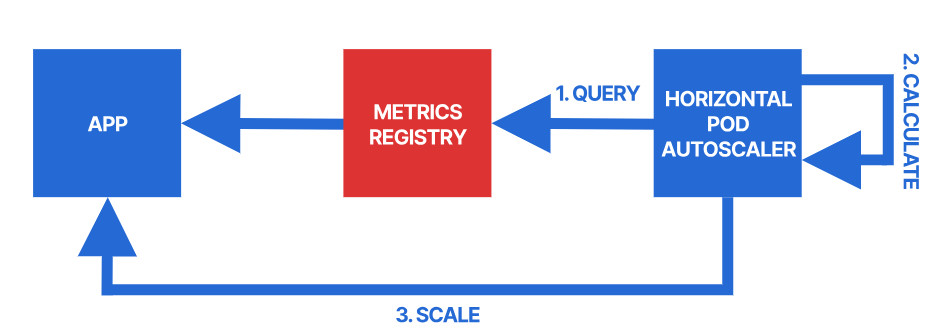
\includegraphics[scale=0.65]{images/phat/metrics_registry.jpg}
    \caption{Horizontal Pod Autoscaler queries flow}
  \end{center}
\end{figure}
Metrics Registry là vị trí trung tâm trong cluster nơi các metrics (dưới bất kỳ hình thức nào) được hiển thị cho clients (Horizontal Pod Autoscaler là một trong những ứng dụng clients này).

Mục đích Metrics Registry là cung cấp giao diện chuẩn cho client truy vấn các metrics.

Interface của Metrics Registry bao gồm 03 API riêng biệt:
\begin{itemize}
    \item The Resource Metrics API
    \item The Custom Metrics API
    \item The External Metrics API
\end{itemize}
\begin{figure}[H]
  \begin{center}
    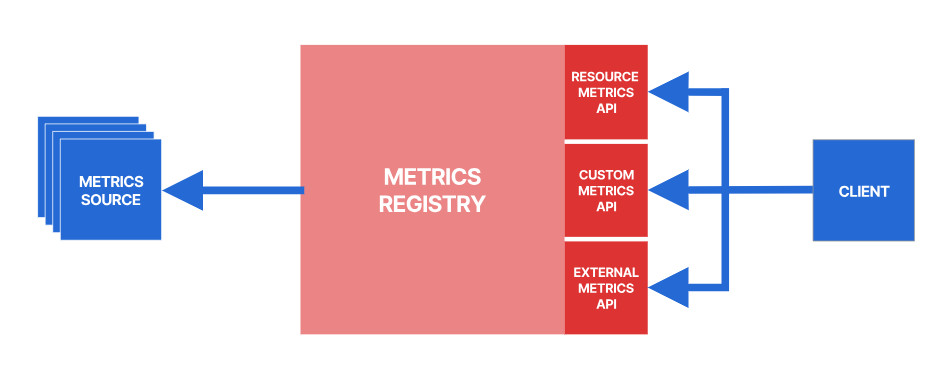
\includegraphics[scale=0.75]{images/phat/metrics_registry_API.jpg}
    \caption{Metrics Registry Interfaces}
  \end{center}
\end{figure}
Các API này được thiết kế để phục vụ các loại metrics khác nhau:
\begin{itemize}
    \item Resource Metrics API: số liệu sử dụng tài nguyên được xác định trước (CPU và bộ nhớ) của Pod và Node.
    \item Custom Metrics API: số liệu tùy chỉnh được liên kết với đối tượng nằm bên trong Kubernetes cluster.
    \item External Metrics API: số liệu tùy chỉnh được liên kết với đối tượng nằm bên ngoài Kubernetes cluster.
\end{itemize}
Vì vậy, để autoscale cho một ứng dụng, nhiệm vụ của chúng ta không chỉ là xác định cấu hình Horizontal Pod Autoscaler mà cũng phải hiển thị metrics mong muốn của mình thông qua Metric Registry.\\[0.5cm]
Đối với mỗi Metric API, chúng ta cần có Metric API Server tương ứng và chúng ta cần định cấu hình cho nó để hiển thị một metric cụ thể thông qua Metric API.\\[0.5cm]
Hơn nữa, chúng ta cần một Metrics Collector để thu thập các metrics mong muốn từ các nguồn (ví dụ: từ Pod của ứng dụng) và cung cấp chúng cho Metric API Server.
\begin{figure}[H]
  \begin{center}
    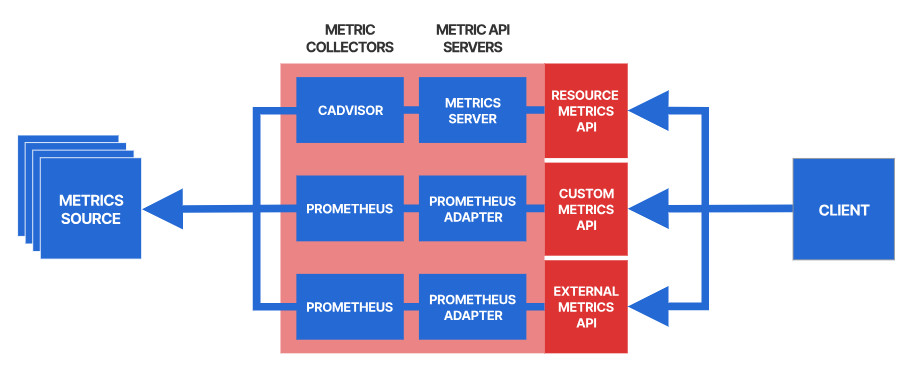
\includegraphics[scale=0.80]{images/phat/metric_registry_detail.jpg}
    \caption{Metrics Registry components}
  \end{center}
\end{figure}
Vì vậy, để expose metric thông qua một trong các API Metrics, chúng ta phải thực hiện các bước sau:
\begin{itemize}
    \item Cài đặt Metrics Collector (ví dụ: Prometheus) và định cấu hình nó để thu thập metric mong muốn (ví dụ: từ Pod của ứng dụng của bạn).
    \item Cài đặt Metric API Server (ví dụ: Prometheus Adapter) và định cấu hình nó để hiển thị từ Metrics collector thông qua Metrics API tương ứng.
\end{itemize}
$\ast$ \textbf{KEDA} sẽ hoạt động với vai trò như một Metric API Server, dùng để biên dịch các metric nhận được từ external server về các dạng dữ liệu mà HPA có thể hiểu được để tiến hành scale thông qua HPA. Như vậy khi sử dụng KEDA thì chúng ta sẽ không cần phải sử dụng Metrics Server từ K8s. Với KEDA chúng ta có 1 khái niệm là \textit{ScaledObject}, khi tạo ScaleObject nó là một phiên bản mở rộng của HPA để thực hiện việc scale pod.
\subsection{Các công nghệ được sử dụng}
\subsubsection{Prometheus}
% TODO: Các phần này cần tự tìm thêm các nguồn khác để tìm hiểu
\textbf{a. Định nghĩa \footnote{https://www.tigera.io/learn/guides/prometheus-monitoring/prometheus-kubernetes}}\\[0.5cm]
Prometheus là một dịch vụ theo dõi và cảnh báo về hệ thống. Prometheus rất thích hợp với những hệ thống Microservices và có các dịch vụ Listening. Một hệ thống theo dõi chủ động như Prometheus sẽ giúp người quản trị phát hiện sớm những dấu hiệu cảnh báo xấu.\\[0.5cm]
Đối với những công việc liên quan đến Queue Job, mối nguy cơ luồng xử lý bị loop hoặc stop rất lớn. Lý do có thể đến từ tài nguyên phần cứng hoặc phần mềm được cài đặt không chính xác. Khi đó việc xem log của dịch vụ đó rất khó hoặc phụ thuộc vào may mắn. Với Prometheus các thông tin luôn được cập nhật và khi xảy ra lỗi, chúng ta vẫn có thể xem lại dữ liệu theo dõi một cách dễ dàng qua API của Prometheus.\\[0.5cm]
\textbf{b. Kiến trúc Prometheus \footnote{https://www.devopsschool.com/blog/what-is-prometheus-and-how-it-works}}

\begin{figure}[H]
  \begin{center}
    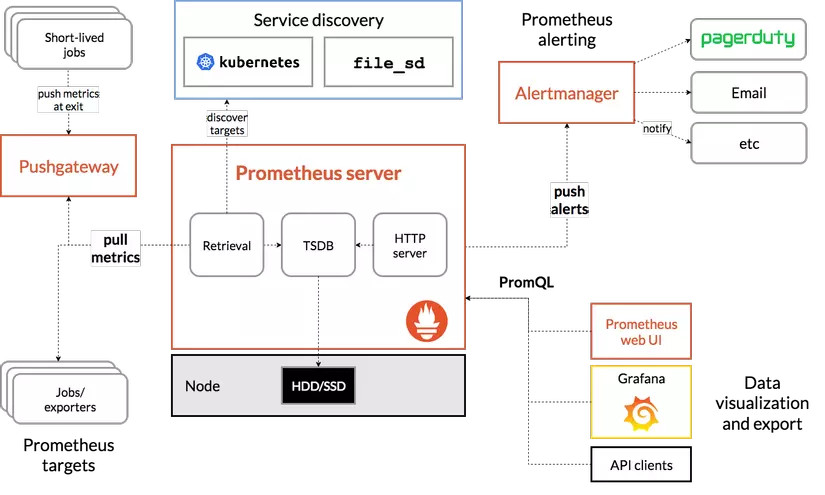
\includegraphics[scale=0.45]{images/phat/prometheus_architecture.jpg}
    \caption{Kiến trúc Prometheus}
  \end{center}
\end{figure}
\textbf{Các thành phần của hệ thống}\\[0.5cm]
\indent Có thể chia kiến trúc Prometheus thành 03 thành phần chính sau: 
\begin{enumerate}
    \item Prometheus Server
    \item Alert Manager
    \item Grafana
\end{enumerate}
\indent Cụ thể các thành phần chi tiết như sau:
\begin{itemize}
    \item \textbf{Prometheus Server}: thành phần chính thu thập, xử lý và lưu trữ dữ liệu chuỗi thời gian (time-series data).
    Nó chủ động liên tục lấy dữ liệu từ các điểm cuối (endpoints) của các dịch vụ và ứng dụng để thu thập thông tin về các metric.
    Dữ liệu thu thập được được lưu trữ tại máy chủ Prometheus.
    \item \textbf{Push Gateway Prometheus}: sử dụng để hỗ trợ các job có thời gian thực hiện ngắn (tạm thời). Đơn giản là các tác vụ công việc này không tồn tại lâu đủ để Prometheus chủ động lấy dữ liệu. Vì vậy là mà các dữ liệu chỉ số (metric) sẽ được đẩy về Push Gateway rồi đẩy về Prometheus Server.
    \item \textbf{Jobs/Exporters}: hỗ trợ giám sát các dịch vụ hệ thống và gửi về Prometheus theo chuẩn Prometheus mong muốn.
    \item \textbf{AlertManager}: dịch vụ quản lý, xử lý các cảnh báo (alert).
    \item \textbf{TSDB \textit{(cơ sở dữ liệu chuỗi thời gian)}}: Prometheus sử dụng TSDB để lưu trữ tất cả dữ liệu một cách hiệu quả. Theo mặc định, tất cả dữ liệu được lưu trữ cục bộ. Tuy nhiên, để tránh single point of failure, có các tùy chọn tích hợp bộ lưu trữ từ xa cho Prometheus TSDB.
\end{itemize}
\textbf{c. Prometheus WorkFlow \footnote{https://prometheus.io/docs/introduction/overview/\#architecture}}
\begin{itemize}
    \item \textbf{Thu Thập Metric}
    \begin{itemize}
        \item Prometheus chủ động liên tục lấy dữ liệu từ các mục tiêu bằng cách gửi các yêu cầu HTTP đến các điểm cuối của chúng (thường là /metrics).
        \item Dữ liệu thu thập được được lưu trữ tại máy chủ Prometheus.
    \end{itemize}
    \item \textbf{Lưu trữ dữ liệu}
    \begin{itemize}
        \item Prometheus lưu trữ dữ liệu chuỗi thời gian tại máy chủ. Định dạng lưu trữ được tối ưu hóa để truy vấn và thống kê nhanh chóng.
    \end{itemize}
    \item \textbf{Truy vấn và ngôn ngữ biểu diễn (PromQL):}
    \begin{itemize}
        \item Prometheus cung cấp một ngôn ngữ truy vấn mạnh mẽ (PromQL) cho việc truy vấn và tổng hợp dữ liệu chuỗi thời gian.
        \item Toán tử, hàm và bộ lựa chọn cho phép người dùng biểu diễn các truy vấn phức tạp và tạo bảng điều khiển tùy chỉnh.
    \end{itemize}
    \item \textbf{Cảnh báo}
    \begin{itemize}
        \item Prometheus có thể định nghĩa các quy tắc cảnh báo dựa trên biểu diễn PromQL. Khi một quy tắc cảnh báo được kích hoạt, một cảnh báo được gửi đến Alertmanager.
        \item Alertmanager sau đó xử lý và chuyển tiếp cảnh báo dựa trên các tuyến đường và ứng dụng thông báo đã được cấu hình.
    \end{itemize}
    \item \textbf{Trực quan hóa}
    \begin{itemize}
        \item Grafana (một plugin của Prometheus) thường được sử dụng như một công cụ trực quan để tạo bảng điều khiển cho các metric của Prometheus. Grafana hỗ trợ Prometheus như một nguồn trực quan hóa dữ liệu bằng biểu đồ và bảng biểu.
    \end{itemize}
\end{itemize}
\subsubsection{KEDA}
% TODO: Các phần này cần tự tìm thêm các nguồn khác để tìm hiểu
\textbf{a. Định nghĩa \footnote{https://KEDA.sh/docs/2.12/concepts/}}\\[0.5cm]
KEDA \textit{(Kubernetes-Based Event-Driven Autoscaler)} là một Kubernetes-based Event Driven Autoscaler. Với KEDA, chúng ta có thể điều chỉnh quy mô của bất kỳ container nào trong Kubernetes dựa trên số lượng sự kiện (event) cần được xử lý.\\[0.5cm]
KEDA là một thành phần nhẹ và đơn mục đích có thể được thêm vào bất kỳ Kubernetes cluster nào. KEDA hoạt động cùng với các thành phần Kubernetes tiêu chuẩn như Horizontal Pod Autoscaler và có thể mở rộng chức năng mà không cần ghi đè hoặc sao chép. Với KEDA, bạn có thể ánh xạ rõ ràng các ứng dụng bạn muốn sử dụng quy mô theo sự kiện, trong khi các ứng dụng khác vẫn tiếp tục hoạt động. Điều này làm cho KEDA trở thành một lựa chọn linh hoạt và an toàn để chạy cùng với bất kỳ ứng dụng hoặc Kubernetes framework nào khác.\\[0.5cm]
\textbf{b. Kiến trúc \footnote{https://devtron.ai/blog/introduction-to-kubernetes-event-driven-autoscaling-KEDA/}}
 
\begin{figure}[H]
  \begin{center}
    \includegraphics[scale=0.32]{images/phat/KEDA Architecture.jpg}
    \caption{Kiến trúc KEDA}
  \end{center}
\end{figure}

\textbf{Các thành phần chính}
\begin{itemize}
    \item \textbf{Event sources}\\
    Đây là các nguồn kích hoạt/sự kiện bên ngoài mà KEDA sử dụng để thay đổi số lượng nhóm. Prometheus, RabbitMQ và Apache Pulsar là một số ví dụ về nguồn sự kiện.
    \item \textbf{Scalers}\\
    Các nguồn sự kiện được giám sát bằng cách sử dụng công cụ chia tỷ lệ, công cụ này tìm nạp số liệu và kích hoạt quy mô Deployments hoặc Jobs dựa trên các sự kiện.
    \item \textbf{Metrics adapter}\\
    Metrics adapter lấy số liệu từ bộ chia tỷ lệ và chuyển đổi hoặc điều chỉnh chúng thành dạng mà thành phần HPA/bộ điều khiển có thể hiểu được.
    \item \textbf{Controller}\\
    Controller hoạt động dựa trên các số liệu do bộ điều hợp cung cấp và mang lại trạng thái triển khai mong muốn được chỉ định trong ScaledObject.
\end{itemize}
\textbf{c. Cách thức hoạt động}\\[0.5cm]
KEDA hoạt động bằng cách tương tác với Kubernetes API và sử dụng các adapters để kết nối và theo dõi các nguồn sự kiện bên ngoài hệ thống Kubernetes. Dưới đây là một mô tả tổng quan về cách KEDA hoạt động:
\begin{itemize}
    \item \textbf{Triển Khai KEDA}
    \begin{itemize}
        \item KEDA được triển khai trên cụm Kubernetes như một Operator hoặc thông qua các tài nguyên Kubernetes tiêu chuẩn.
    \end{itemize}
    \item \textbf{Sự Kiện và adapter}
    \begin{itemize}
        \item KEDA sử dụng các adapters để theo dõi các nguồn sự kiện bên ngoài hệ thống Kubernetes. Các adapters này có thể là các thành phần được tích hợp sẵn để xử lý các loại sự kiện cụ thể.
        \item Ví dụ: Nếu bạn muốn mở rộng dựa trên kích thước hàng đợi RabbitMQ, bạn có thể sử dụng adapter RabbitMQ của KEDA.
    \end{itemize}
    \item \textbf{Tích Hợp với Pod Scaler}
    \begin{itemize}
        \item Pod Scaler là một thành phần quan trọng của KEDA và chịu trách nhiệm về việc mở rộng (hoặc giảm) số lượng pods dựa trên sự kiện được theo dõi.
        \item Khi có sự kiện xảy ra, Pod Scaler sẽ quyết định xem cần mở rộng, giảm số lượng pods, hoặc duy trì tình trạng hiện tại.
    \end{itemize}
    \item \textbf{Kết Nối với Kubernetes API}
    \begin{itemize}
        \item Pod Scaler tương tác với Kubernetes API để điều chỉnh số lượng pods. Nó có thể thay đổi các ReplicaSets hoặc Deployments để tăng giảm quy mô.
    \end{itemize}
    \item \textbf{Chia Sẻ Thông Tin với Metrics Server}
    \begin{itemize}
        \item Pod Scaler thông tin về trạng thái hiện tại và các quyết định của mình với Metrics Server. Metrics Server cung cấp thông tin về hiệu suất và trạng thái của các pods.
    \end{itemize}
    \item \textbf{Môi Trường Linh Hoạt và Quản Lý Tài Nguyên}
    \begin{itemize}
        \item KEDA cung cấp một môi trường linh hoạt cho việc xử lý sự kiện và quản lý tài nguyên. Nó có thể mở rộng dựa trên nhiều loại sự kiện và chia sẻ nguồn lực giữa nhiều ứng dụng.
    \end{itemize}
\end{itemize}
Tóm lại, KEDA hoạt động như một thành phần giám sát và quản lý tài nguyên mạnh mẽ trong môi trường Kubernetes. Nó tương tác với các nguồn sự kiện bên ngoài và tự động điều chỉnh số lượng pods của ứng dụng để đảm bảo rằng tài nguyên được triển khai hiệu quả và hiệu suất tốt nhất.
\subsubsection{K6}
% TODO: Các phần này cần tự tìm thêm các nguồn khác để tìm hiểu
\textbf{a. Bài toán đặt ra \footnote{https://techmaster.vn/posts/36882/performance-testing-voi-k6}}\\[0.5cm]
Giả sử chúng ta code 1 API mà khi dùng postman tạo request thì thấy cũng có response. Tuy nhiên, sau khi đưa vào sử dụng thì ngày nào cũng thấy bị log lỗi do request gửi vào liên tục, dẫn đến tình trạng cao tải, thành ra tính năng thì có, nhưng gần như không dùng được, vì vậy để giúp xác định tắc nghẽn trong một hệ thống, thiết lập một đường cơ sở để kiểm thử trong tương lai, hỗ trợ điều chỉnh hiệu suất hiệu quả, xác định sự phù hợp mục tiêu và yêu cầu hiệu suất, và thu thập dữ liệu hoạt động liên quan khác để giúp các bên liên quan đưa ra quyết định liên quan đến chất lượng chung của các ứng dụng đang được kiểm thử thì việc dùng performance testing là một lựa chọn tối ưu.\\[0.5cm]
Performance Testing là một loại kiểm thử nhằm xác định mức độ đáp ứng, băng thông, độ tin cậy và/hoặc khả năng mở rộng của hệ thống dưới một khối lượng làm việc/truy cập nhất định.\\[0.5cm]
Hiện tại có rất nhiều công cụ hỗ trợ kiểm thử hiệu năng như Jmeter, Grinder, LoadComplete, K6, v.v.\\[0.5cm]
\textbf{b. Định nghĩa \footnote{https://anhdevhamhoc.com/view/16-k6-inovative-and-effective-performace-testing-tool}}\\[0.5cm]
K6 là một công cụ mã nguồn mở được đặc biệt thiết kế để thực hiện kiểm tra hiệu suất và khả năng chịu tải các ứng dụng web và API. Do Load Impact phát triển, K6 nhằm mục tiêu đơn giản hóa quá trình kiểm tra hiệu năng và cung cấp kết quả đáng tin cậy, giúp các nhà phát triển và quản trị hệ thống đưa ra các quyết định thông minh về hiệu suất của ứng dụng.\\[0.5cm]
\textbf{c. Ưu điểm của K6}
\begin{itemize}
    \item \textbf{Sử dụng JavaScript làm ngôn ngữ lập trình}\\
    K6 được xây dựng bằng JavaScript, một ngôn ngữ lập trình phổ biến và dễ tiếp cận. Điều này giảm thiểu thời gian học và cho phép các nhà phát triển sử dụng kiến thức JavaScript hiện có để tạo ra các kịch bản kiểm tra hiệu suất một cách hiệu quả.
    \item \textbf{Dễ cài đặt và sử dụng}\\
    K6 có cấu trúc đơn giản và rõ ràng, giúp người dùng nhanh chóng cài đặt và bắt đầu tạo các bài kiểm tra. Chỉnh sửa và xem xét mã cũng trở nên dễ dàng, tiết kiệm thời gian và tăng hiệu suất công việc.
     \item \textbf{Kiểm tra tải đơn giản}\\
     K6 hỗ trợ kiểm tra tải tập trung (stress testing), kiểm tra tải phân tán (load testing), và kiểm tra hiệu suất chức năng (functional testing). Điều này giúp người dùng có cái nhìn tổng quan về hiệu năng ứng dụng trong nhiều tình huống khác nhau.
     \item \textbf{Hỗ trợ đa nền tảng}\\
     K6 chạy trên nhiều nền tảng, bao gồm Windows, macOS và Linux. Điều này cho phép người dùng thực hiện các bài kiểm tra từ các môi trường khác nhau một cách dễ dàng.
     \item \textbf{Tích hợp linh hoạt và thư viện mở rộng}:\\
     K6 hỗ trợ nhiều thư viện mở rộng bổ sung, giúp người dùng mở rộng khả năng kiểm tra của mình. Nó cũng tích hợp tốt với các công cụ phổ biến như Grafana và InfluxDB để hiển thị kết quả kiểm tra hiệu suất một cách trực quan.
     \item \textbf{Hiệu suất mạnh mẽ}\\
     K6 được thiết kế để xử lý số lượng lớn yêu cầu đồng thời và đáp ứng trong thời gian thực. Điều này giúp các chuyên gia hiệu suất thực hiện kiểm tra trong các điều kiện khắc nghiệt mà vẫn duy trì độ chính xác cao.
\end{itemize}
\subsection{Các bước thực hiện}
\noindent Sau khi đã tìm hiểu các thành phần công nghê sẽ được sử dụng, ta sẽ cài đặt chúng vào Kubernetes cluster. Để có thể scale một service theo request, ta cần hiện thực các dịch vụ sau vào cluster:
\begin{itemize}
  \item Prometheus server
  \item Keda runtime.
\end{itemize}
Các bước thực hiện cụ thể sẽ được mô tả ở các tiểu mục bên dưới.
\subsubsection{Hiện thực prometheus server}
\noindent Để hiện thực Prometheus server, ta cần làm theo các bước sau:\footnote{https://devopscube.com/setup-prometheus-monitoring-on-kubernetes/}
% \begin{enumerate}[label=\textbf{Bước \arabic*:}, leftmargin=*]
\begin{itemize}
  \item \textbf{Bước 1: Tạo Namespace và ClusterRole.}\\[0.2cm]
  Ta sẽ tạo một namespace riêng cho Prometheus server và các service đi theo nó, mục đích là để tách biệt chúng ra khỏi các service phục vụ cho các yêu cầu khác của hệ thống.\\[0.2cm]
  Ta tạo namespace \textbf{monitoring} bằng câu lệnh \lstinline|kubectl create namespace monitoring|.\\[0.2cm]
  Sau đó, ta áp dụng config Cluster Role dưới đây vào cluster:
  \begin{lstlisting}[language=yaml]
apiVersion: rbac.authorization.k8s.io/v1
kind: ClusterRole
metadata:
  name: prometheus
rules:
- apiGroups: [""]
  resources:
  - nodes
  - nodes/proxy
  - services
  - endpoints
  - pods
  verbs: ["get", "list", "watch"]
- apiGroups:
  - extensions
  resources:
  - ingresses
  verbs: ["get", "list", "watch"]
- nonResourceURLs: ["/metrics"]
  verbs: ["get"]
---
apiVersion: rbac.authorization.k8s.io/v1
kind: ClusterRoleBinding
metadata:
  name: prometheus
roleRef:
  apiGroup: rbac.authorization.k8s.io
  kind: ClusterRole
  name: prometheus
subjects:
- kind: ServiceAccount
  name: default
  namespace: monitoring

  \end{lstlisting}
  \item \textbf{Bước 2: Tạo Config map để mở rộng cấu hình của Prometheus}\\[0.2cm]
  Prometheus, theo như ở phần trên, có thể đóng rất nhiều vai trò khác nhau trong một hệ thống. Do đó, việc cần điểu chỉnh cấu hình của nó là điều thường xuyên xảy ra. Thay vì cần phải build lại image của Prometheus mỗi khi cấu hình được điều chỉnh, thì nay ta có thể đem những cấu hình đó ra ngoài dưới dạng 1 file config map, từ đó tiết kiệm thời gian áp dụng thay đổi, thay vì phải build lại image, rồi push image lên hub, cuối cùng là kéo về cluster, thì ta chỉ cần khởi động lại prometheus pod là được.\\[0.2cm]
  Cấu hình Config map của prometheus như sau:
  \begin{lstlisting}[language=yaml]
apiVersion: v1
kind: ConfigMap
metadata:
  name: prometheus-server-conf
  labels:
    name: prometheus-server-conf
  namespace: monitoring
data:
  prometheus.rules: |-
    groups:
    - name: devopscube demo alert
      rules:
      - alert: High Pod Memory
        expr: sum(container_memory_usage_bytes) > 1
        for: 1m
        labels:
          severity: slack
        annotations:
          summary: High Memory Usage
  prometheus.yml: |-
    global:
      scrape_interval: 5s
      evaluation_interval: 5s
    rule_files:
      - /etc/prometheus/prometheus.rules
    alerting:
      alertmanagers:
      - scheme: http
        static_configs:
        - targets:
          - "alertmanager.monitoring.svc:9093"
    scrape_configs:
      - job_name: 'node-exporter'
        kubernetes_sd_configs:
          - role: endpoints
        relabel_configs:
        - source_labels: [__meta_kubernetes_endpoints_name]
          regex: 'node-exporter'
          action: keep
      - job_name: 'kubernetes-apiservers'
        kubernetes_sd_configs:
        - role: endpoints
        scheme: https
        tls_config:
          ca_file: /var/run/secrets/kubernetes.io/serviceaccount/ca.crt
        bearer_token_file: /var/run/secrets/kubernetes.io/serviceaccount/token
        relabel_configs:
        - source_labels: [__meta_kubernetes_namespace, __meta_kubernetes_service_name, __meta_kubernetes_endpoint_port_name]
          action: keep
          regex: default;kubernetes;https
      - job_name: 'kubernetes-nodes'
        scheme: https
        tls_config:
          ca_file: /var/run/secrets/kubernetes.io/serviceaccount/ca.crt
        bearer_token_file: /var/run/secrets/kubernetes.io/serviceaccount/token
        kubernetes_sd_configs:
        - role: node
        relabel_configs:
        - action: labelmap
          regex: __meta_kubernetes_node_label_(.+)
        - target_label: __address__
          replacement: kubernetes.default.svc:443
        - source_labels: [__meta_kubernetes_node_name]
          regex: (.+)
          target_label: __metrics_path__
          replacement: /api/v1/nodes/${1}/proxy/metrics
      - job_name: 'kubernetes-pods'
        kubernetes_sd_configs:
        - role: pod
        relabel_configs:
        - source_labels: [__meta_kubernetes_pod_annotation_prometheus_io_scrape]
          action: keep
          regex: true
        - source_labels: [__meta_kubernetes_pod_annotation_prometheus_io_path]
          action: replace
          target_label: __metrics_path__
          regex: (.+)
        - source_labels: [__address__, __meta_kubernetes_pod_annotation_prometheus_io_port]
          action: replace
          regex: ([^:]+)(?::\d+)?;(\d+)
          replacement: $1:$2
          target_label: __address__
        - action: labelmap
          regex: __meta_kubernetes_pod_label_(.+)
        - source_labels: [__meta_kubernetes_namespace]
          action: replace
          target_label: kubernetes_namespace
        - source_labels: [__meta_kubernetes_pod_name]
          action: replace
          target_label: kubernetes_pod_name
      - job_name: 'kube-state-metrics'
        static_configs:
          - targets: ['kube-state-metrics.kube-system.svc.cluster.local:8080']
      - job_name: 'kubernetes-cadvisor'
        scheme: https
        tls_config:
          ca_file: /var/run/secrets/kubernetes.io/serviceaccount/ca.crt
        bearer_token_file: /var/run/secrets/kubernetes.io/serviceaccount/token
        kubernetes_sd_configs:
        - role: node
        relabel_configs:
        - action: labelmap
          regex: __meta_kubernetes_node_label_(.+)
        - target_label: __address__
          replacement: kubernetes.default.svc:443
        - source_labels: [__meta_kubernetes_node_name]
          regex: (.+)
          target_label: __metrics_path__
          replacement: /api/v1/nodes/${1}/proxy/metrics/cadvisor
      - job_name: 'kubernetes-service-endpoints'
        kubernetes_sd_configs:
        - role: endpoints
        relabel_configs:
        - source_labels: [__meta_kubernetes_service_annotation_prometheus_io_scrape]
          action: keep
          regex: true
        - source_labels: [__meta_kubernetes_service_annotation_prometheus_io_scheme]
          action: replace
          target_label: __scheme__
          regex: (https?)
        - source_labels: [__meta_kubernetes_service_annotation_prometheus_io_path]
          action: replace
          target_label: __metrics_path__
          regex: (.+)
        - source_labels: [__address__, __meta_kubernetes_service_annotation_prometheus_io_port]
          action: replace
          target_label: __address__
          regex: ([^:]+)(?::\d+)?;(\d+)
          replacement: $1:$2
        - action: labelmap
          regex: __meta_kubernetes_service_label_(.+)
        - source_labels: [__meta_kubernetes_namespace]
          action: replace
          target_label: kubernetes_namespace
        - source_labels: [__meta_kubernetes_service_name]
          action: replace
          target_label: kubernetes_name
  \end{lstlisting}
  \item \textbf{Bước 3: Tạo một Prometheus Deployment}\\[0.2cm]
  Sau khi chuẩn bị sẵn sàng các dịch vụ hỗ trợ đi kèm, ta có thể khởi tạo một deployment cho Prometheus server theo config dưới đây.
  \begin{lstlisting}[language=yaml]
apiVersion: apps/v1
kind: Deployment
metadata:
  name: prometheus-deployment
  namespace: monitoring
  labels:
    app: prometheus-server
spec:
  replicas: 1
  selector:
    matchLabels:
      app: prometheus-server
  template:
    metadata:
      labels:
        app: prometheus-server
    spec:
      containers:
        - name: prometheus
          image: prom/prometheus
          args:
            - "--config.file=/etc/prometheus/prometheus.yml"
            - "--storage.tsdb.path=/prometheus/"
          ports:
            - containerPort: 9090
          volumeMounts:
            - name: prometheus-config-volume
              mountPath: /etc/prometheus/
            - name: prometheus-storage-volume
              mountPath: /prometheus/
      volumes:
        - name: prometheus-config-volume
          configMap:
            defaultMode: 420
            name: prometheus-server-conf
  
        - name: prometheus-storage-volume
          emptyDir: {}
  \end{lstlisting}
  Khởi tạo thành công, ta có thể nhìn thấy sự xuất hiện của Prometheus pod và deployment ở namespace \textbf{monitoring} như hình dưới.
  \begin{figure}[H]
    \begin{center}
      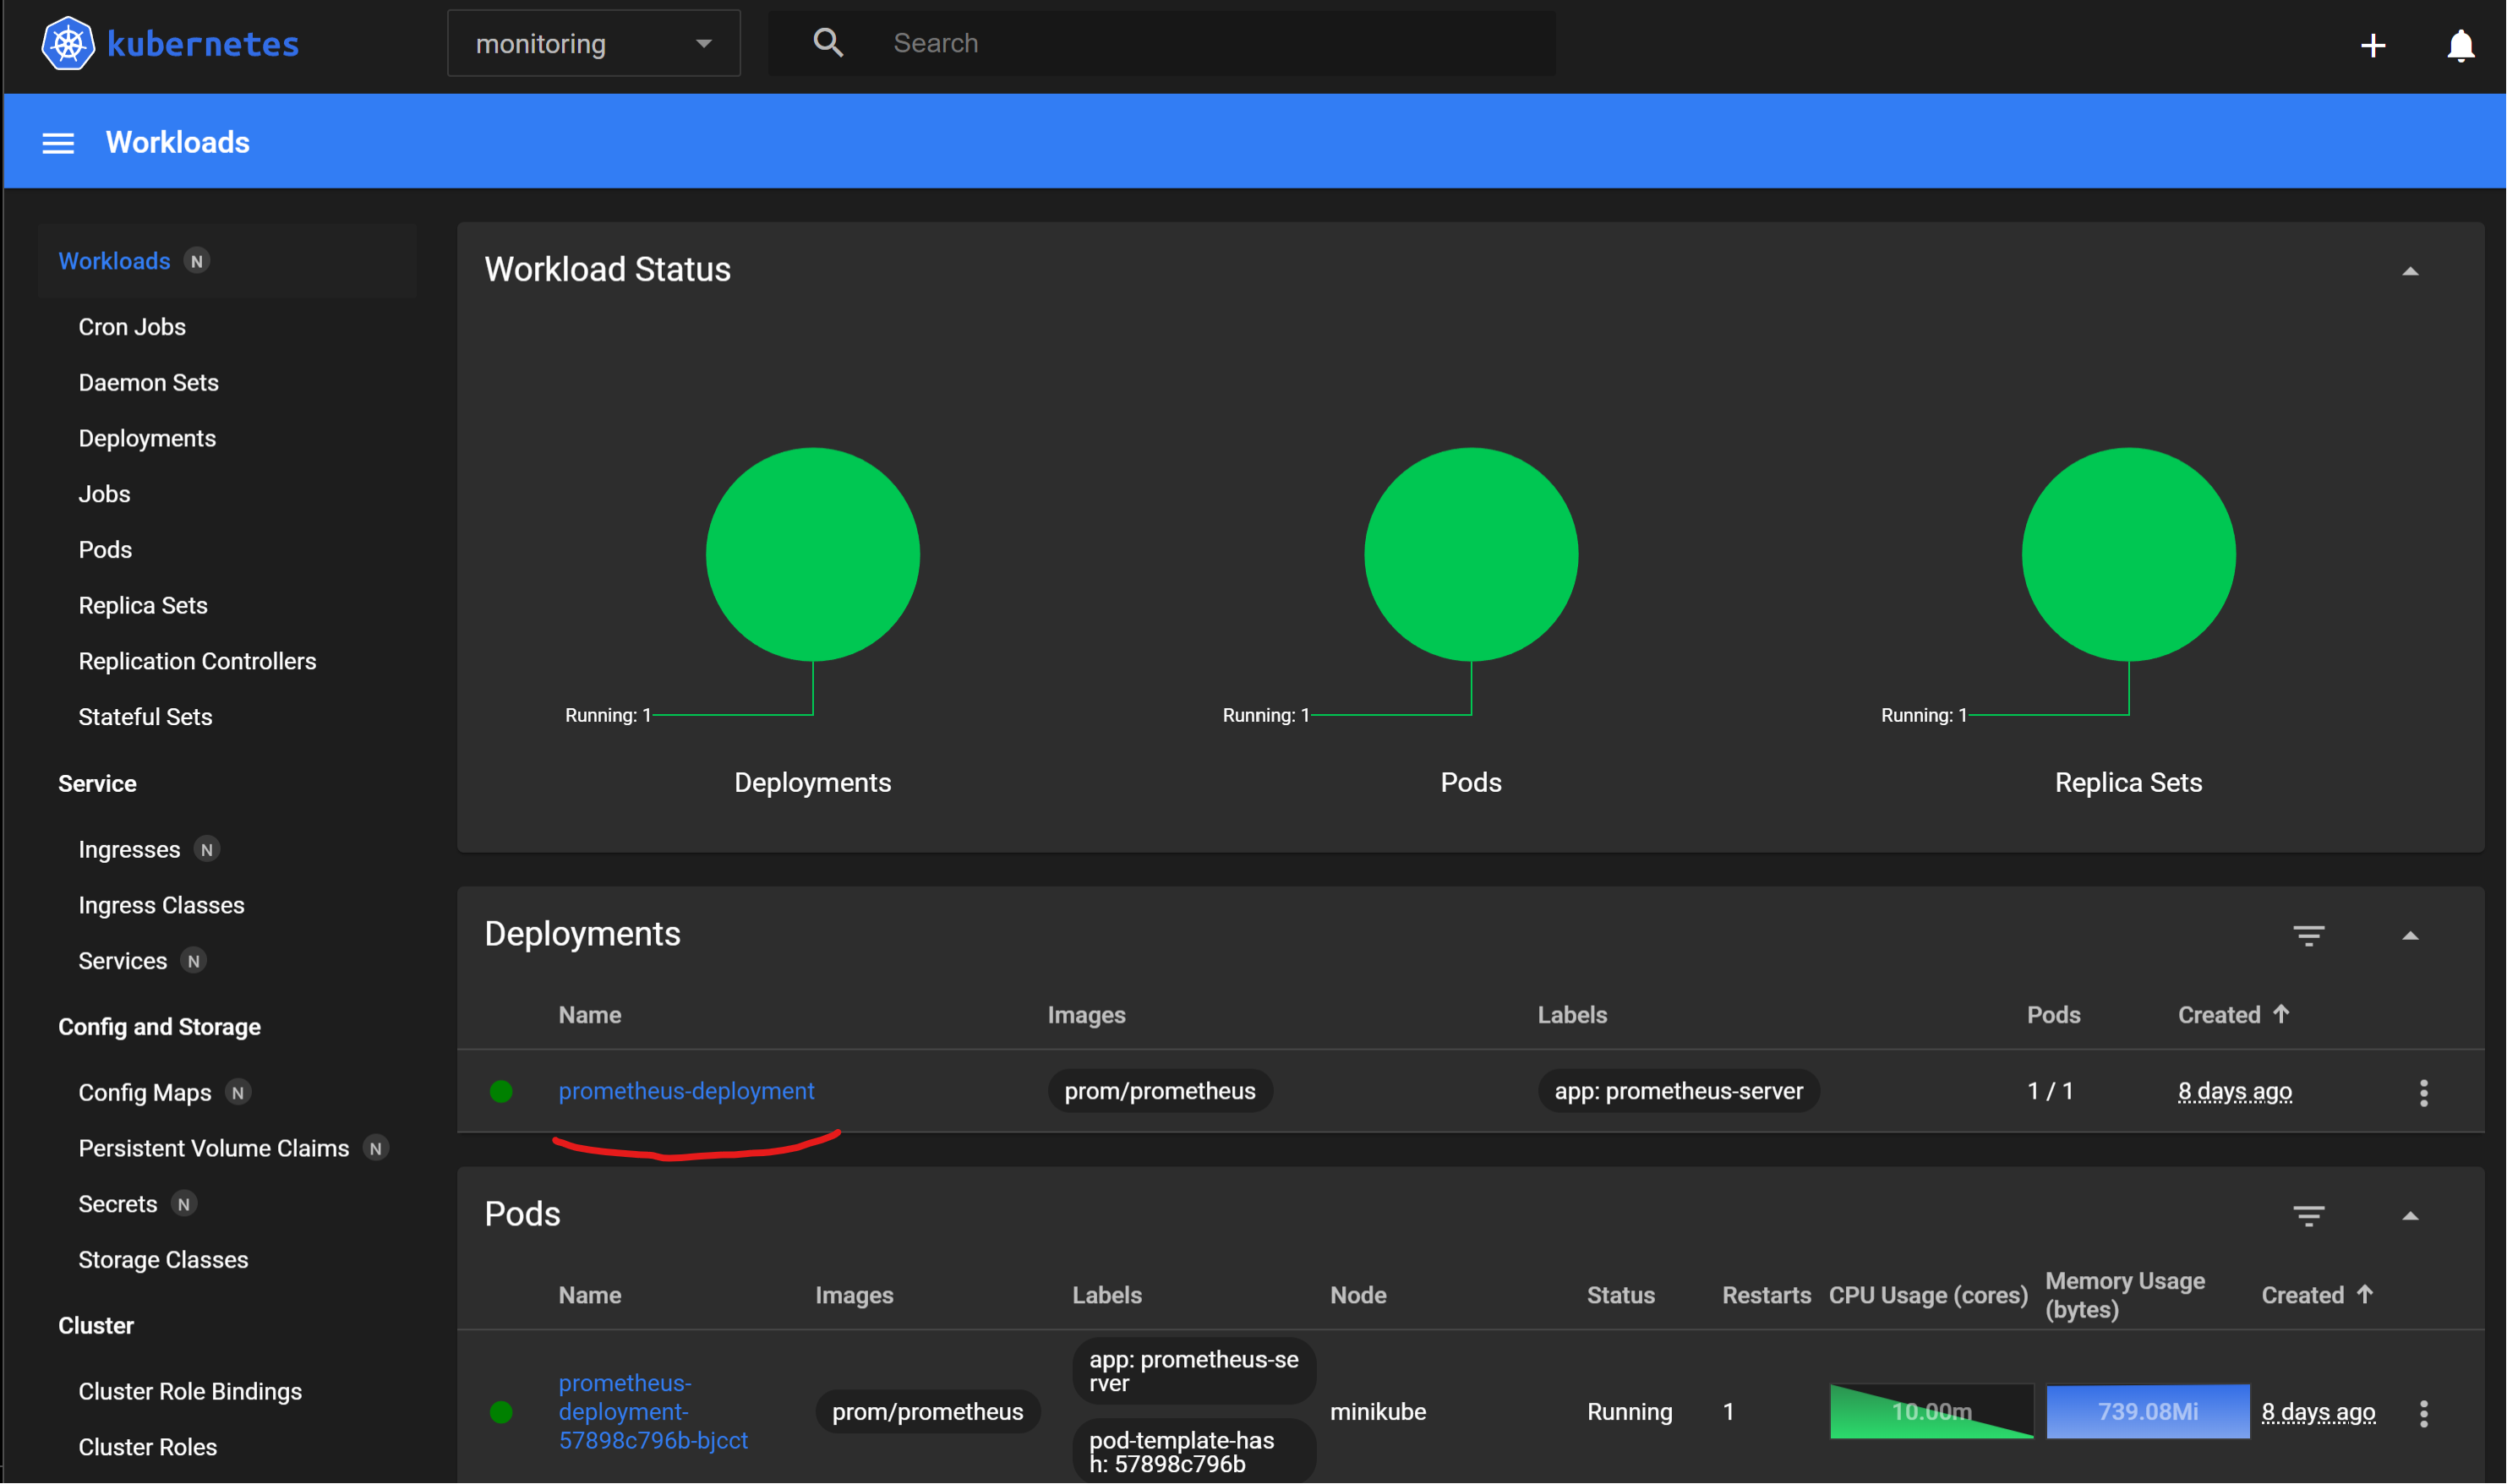
\includegraphics[scale = 0.4]{images/hanh/prometheus-deployment.png}
      \caption{Prometheus pod và deployment được thể hiện ở minikube cluster dashboard}
    \end{center}
    \label{}
  \end{figure}
  \item \textbf{Bước 4: Kết nối tới Prometheus Dashboard}\\[0.2cm]
  Sau khi đã cài đặt đầy đủ Prometheus server và các dịch vụ đi kèm, ta có thể truy cập vào dashboard của Prometheus để xem các thông số. Ví dụ với minikube cluster, ta có thể dùng lệnh \lstinline|minikube service prometheus-service| để mở cổng truy cập, cho phép truy cập từ máy tính của chúng ta vào Prometheus server.
  \begin{figure}[H]
    \begin{center}
      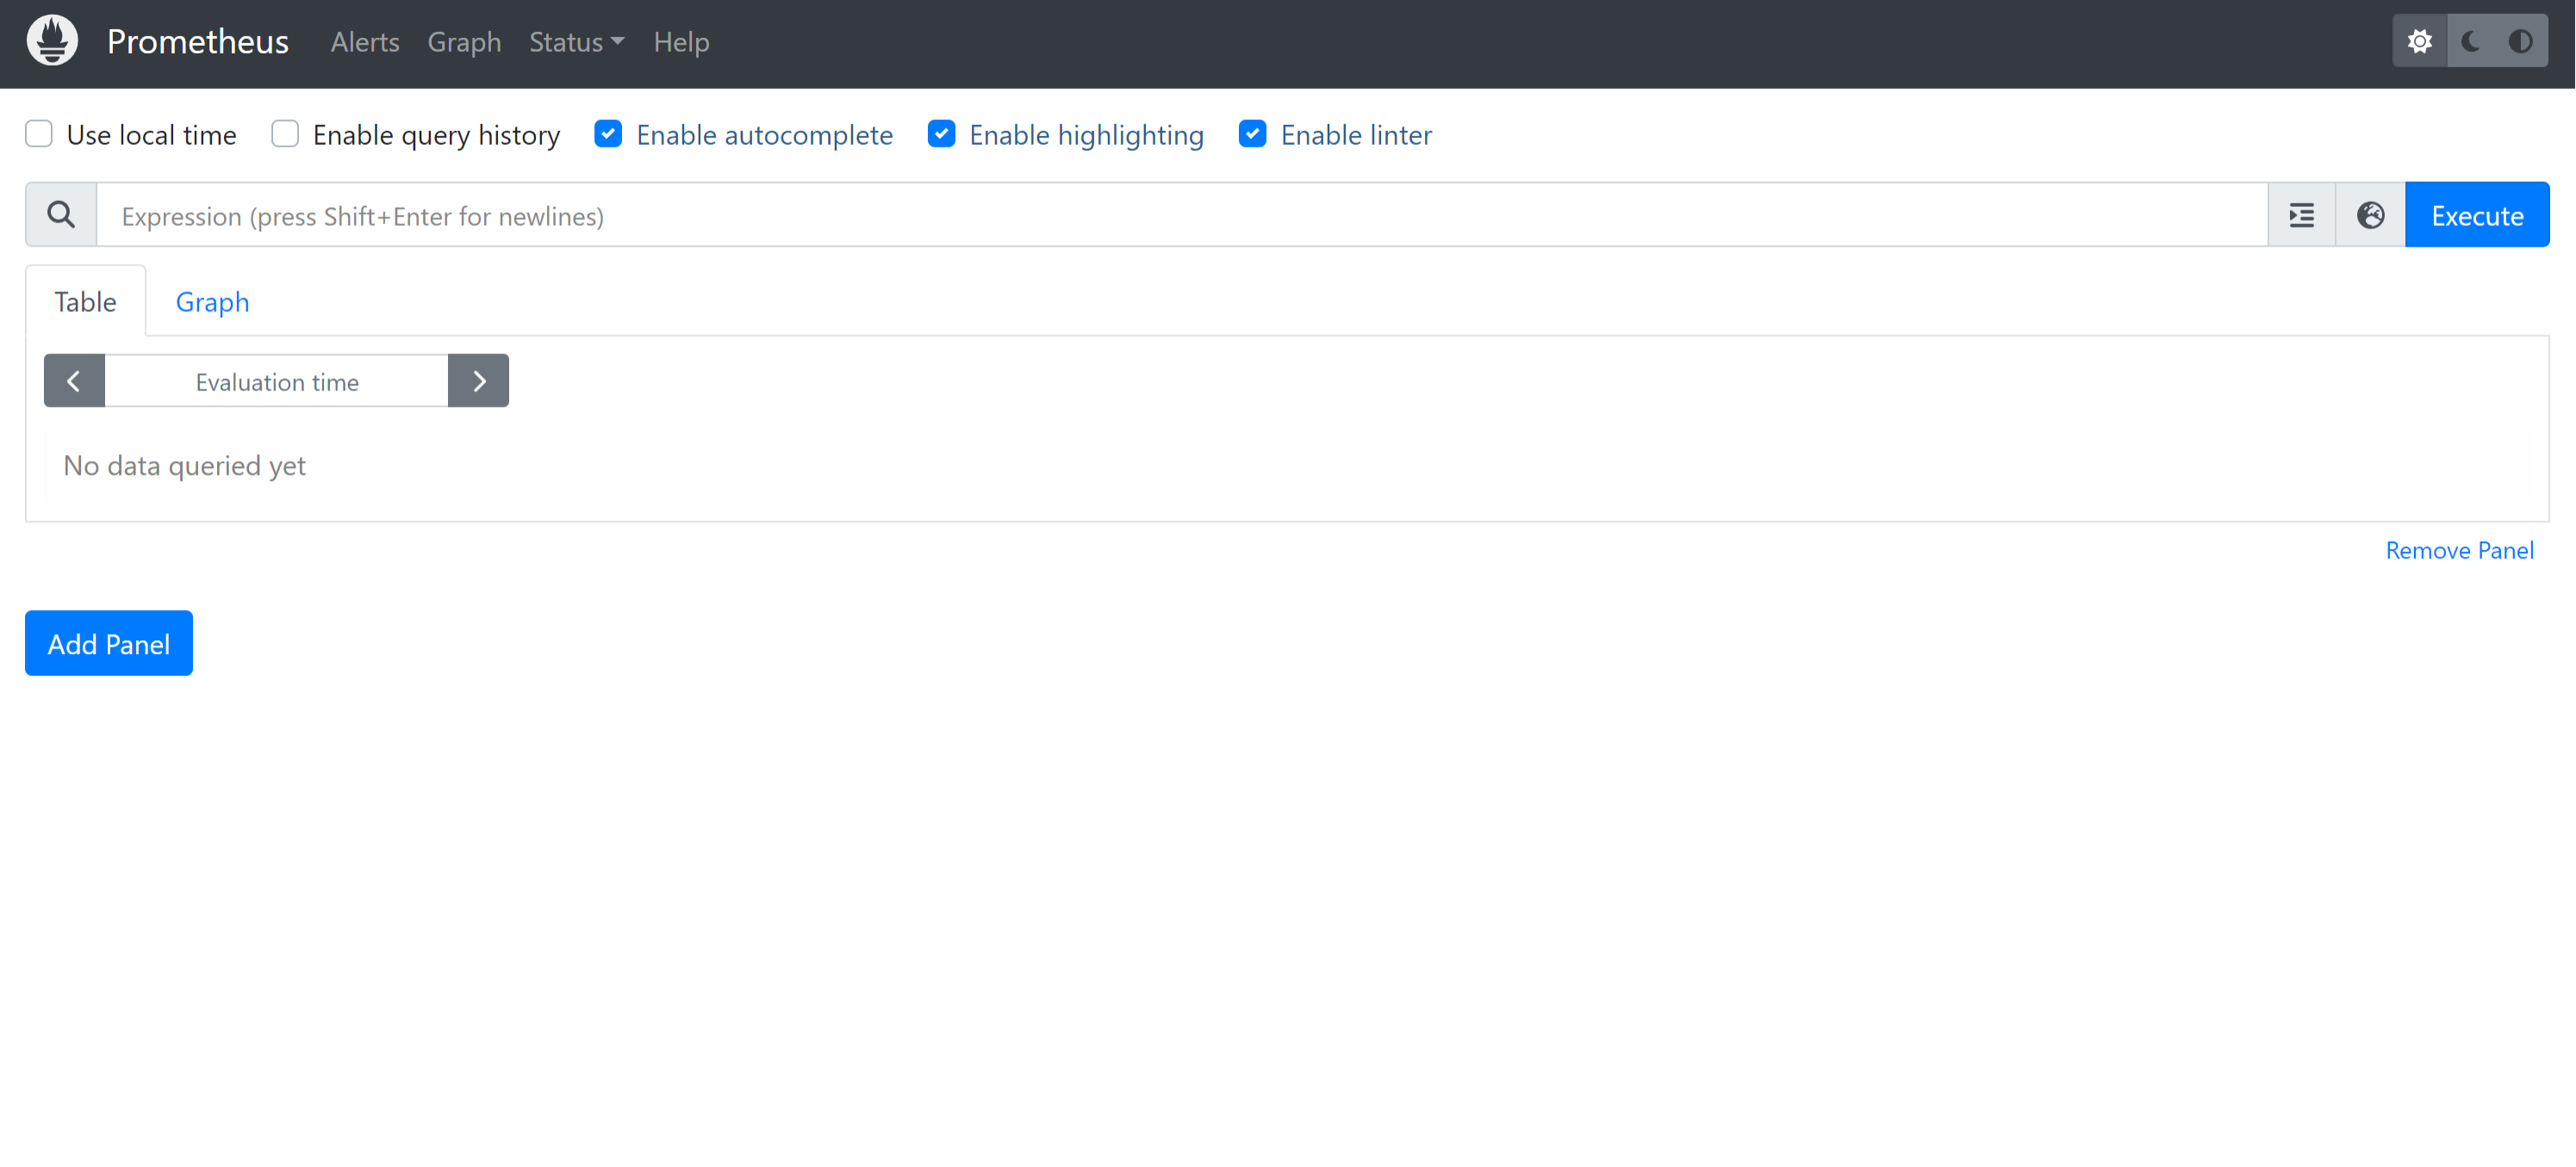
\includegraphics[scale=0.4]{images/hanh/prometheus-dashboard.png}
      \caption{Prometheus dashboard khi vừa mới khởi tạo}
    \end{center}
    \label{}
  \end{figure}

\end{itemize}
\subsubsection{Hiện thực Keda runtime}
\noindent Các ScaledObject của Keda không phải tự nhiên mà có thể vân hành tốt với Kubernetes cluster, mà cần có sư hỗ trợ của keda runtime để có thể vận hành các chức năng cần thiết. Đội ngũ phát triển của Keda đã cung cấp và gói gọn cho chúng ta toàn bộ các cấu hình cần thiết vào trong 1 file cấu hình yaml dài hơn 9700 dòng, mà từ đó ta có thể dễ dàng cài đặt thông qua câu lệnh sau: \lstinline|kubectl apply --server-side -f https://|\lstinline|github.com/kedacore/keda/releases/download/v2.12.1/keda-2.12.1-core.yaml|\\[0.2cm]
Sau khi quá trình cài đặt hoàn tất, ta có thể kiểm tra các dịch vụ đã được cài vào trong cluster thông qua minikube dashboard, namespace \textbf{keda}.
\begin{figure}[H]
  \begin{center}
    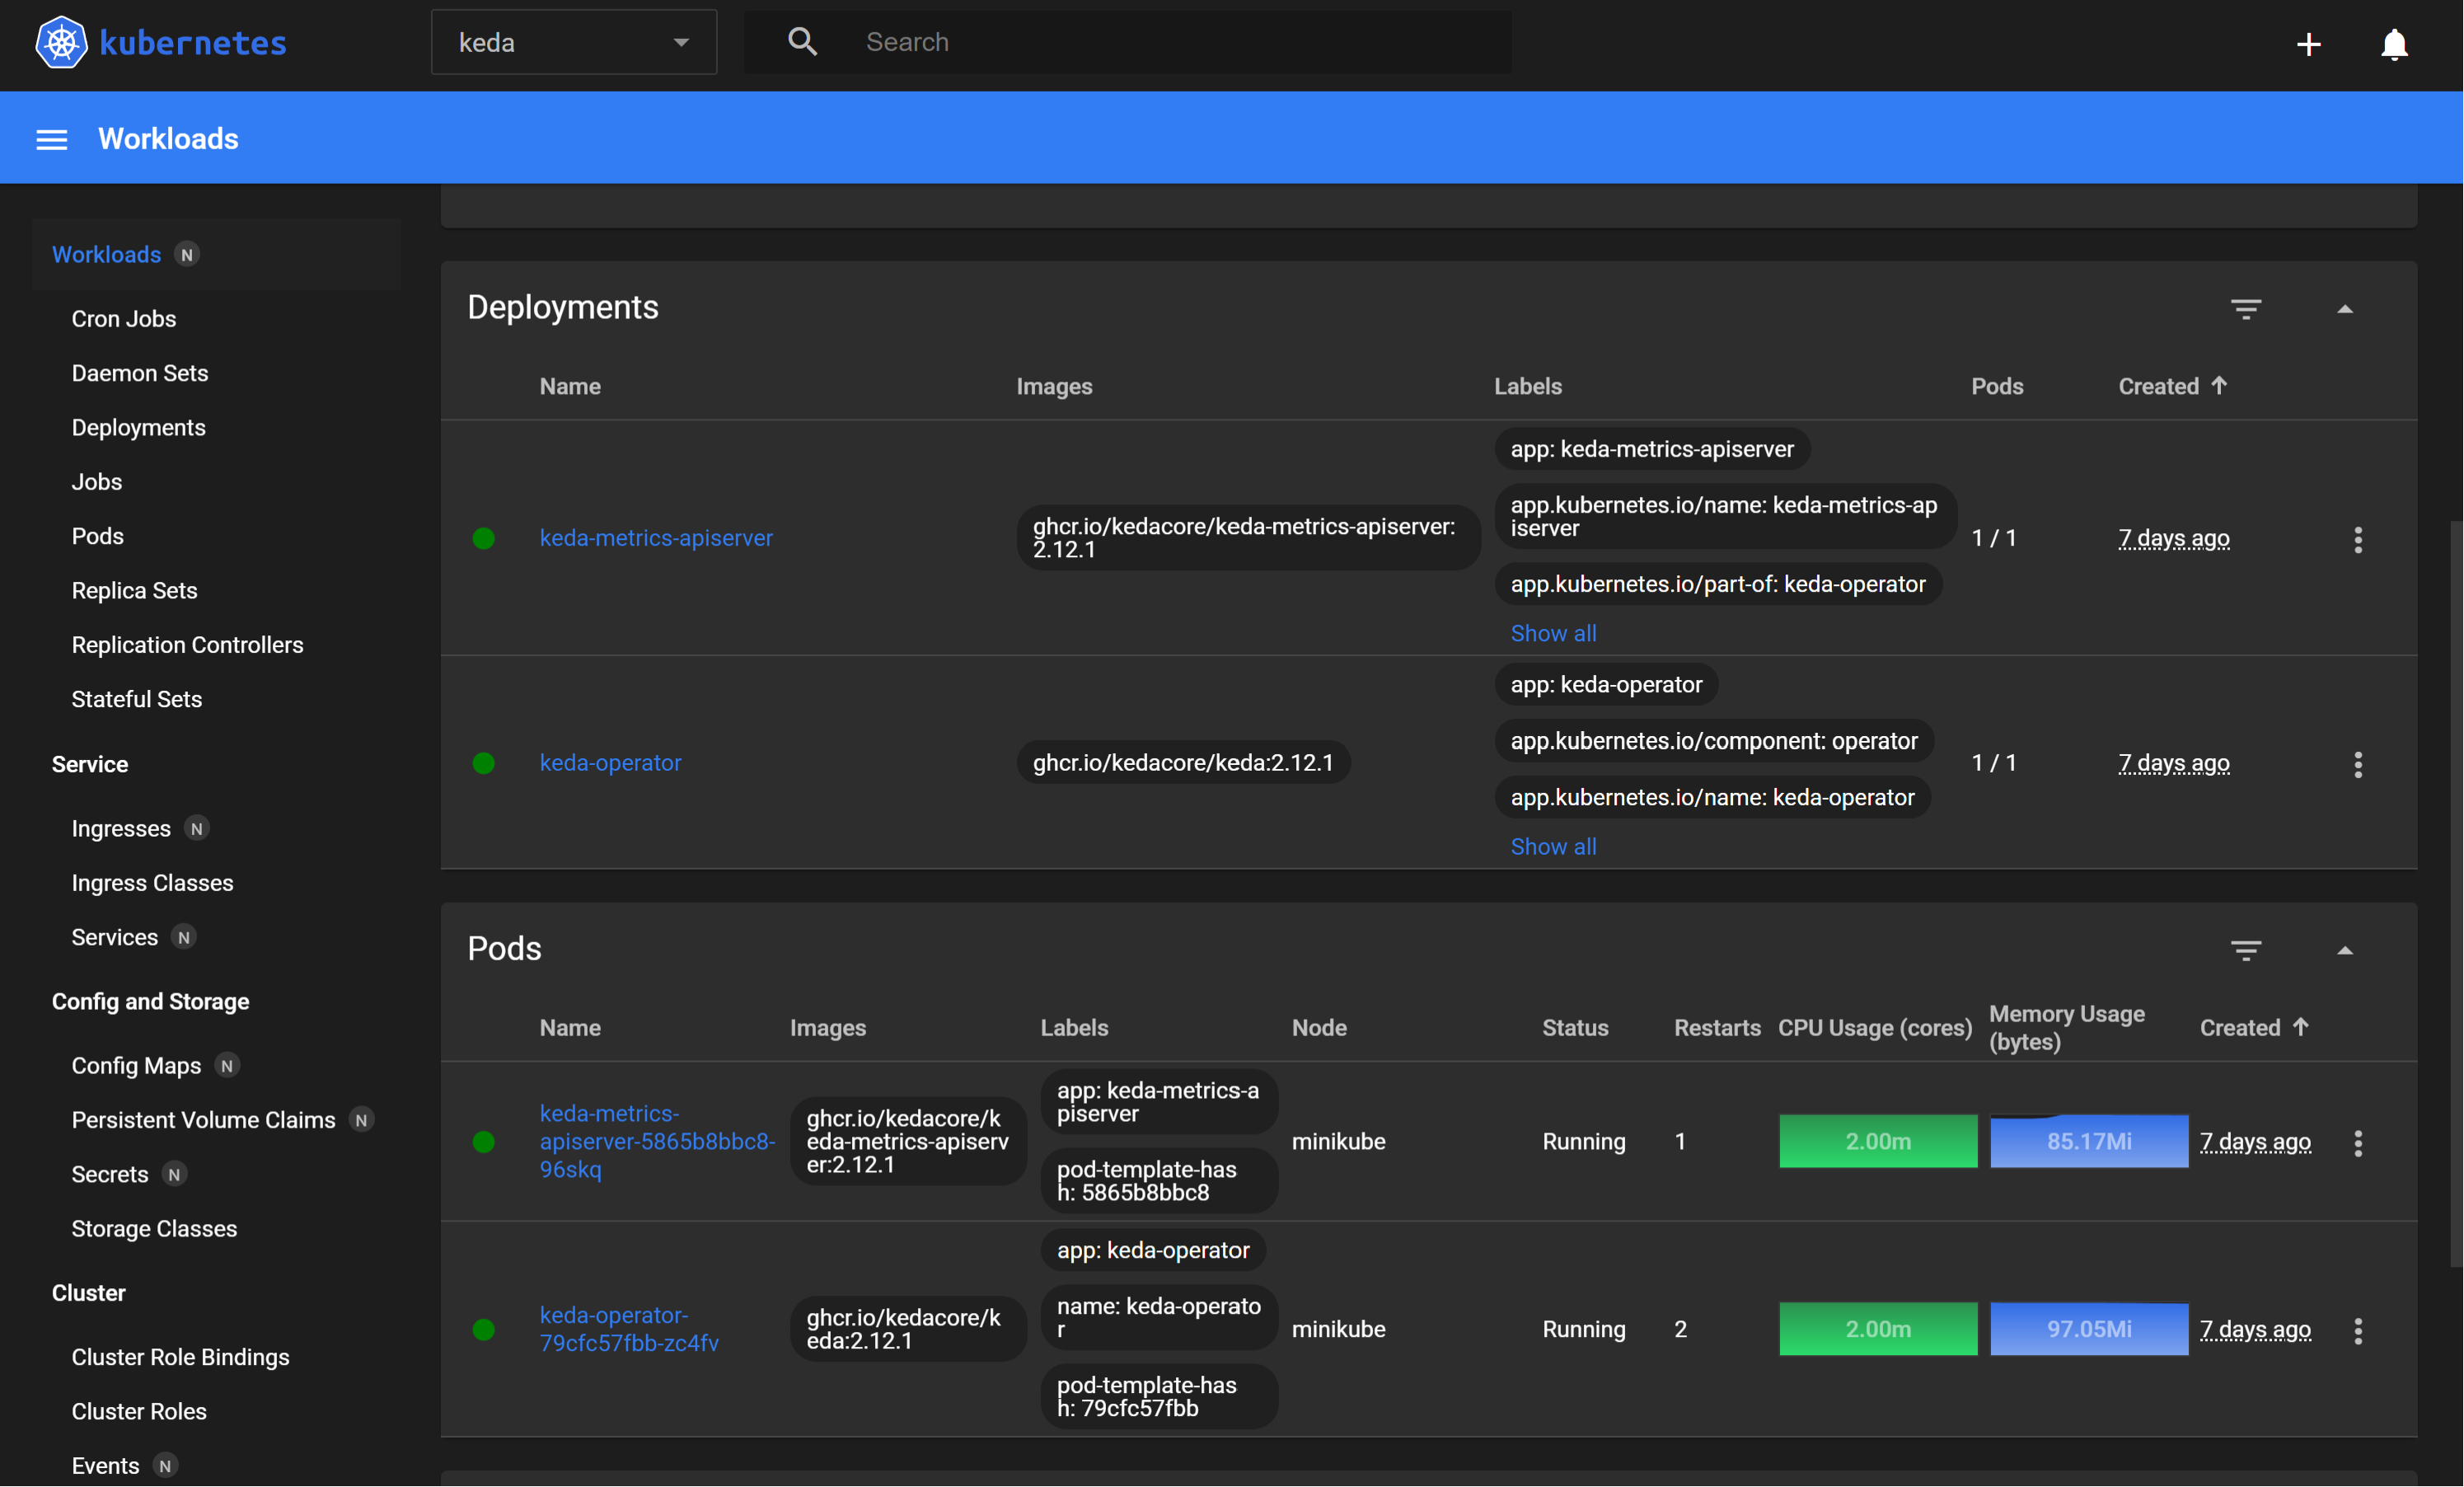
\includegraphics[scale=0.4]{images/hanh/keda-deployment.png}
    \caption{Các deployment và pod phục vụ cho Keda runtime được khởi tạo}
  \end{center}
  \label{}
\end{figure}

\subsubsection{Hiện thực Keda ScaledObject}
\noindent Khi Prometheus server đã sẵn sàng để tiếp nhận thông tin, Keda runtime sẵn sàng cung cấp thông tin đó tới các Keda object thông qua API \lstinline|keda.sh|, thì đó là lúc ta có thể tiến hành cài đặt Keda ScaledObject, nhằm phục vụ cho việc scale theo request của dịch vụ theo cấu hình dưới đây.

\begin{lstlisting}[language=yaml]
apiVersion: keda.sh/v1alpha1
kind: ScaledObject
metadata:
  name: prometheus-scaledobject
  namespace: default
spec:
  scaleTargetRef:
    name: catalog-ms-1-deploy
  pollingInterval: 10  # Optional. Default: 30 seconds
  cooldownPeriod:  15 # Optional. Default: 300 seconds
  minReplicaCount: 1   # Optional. Default: 0
  maxReplicaCount: 10 # Optional. Default: 100
  # fallback:           # Optional. Section to specify fallback options
  #   failureThreshold: 3    # Mandatory if fallback section is included
  #   replicas: 1
  advanced: # Optional. Section to specify advanced options
    horizontalPodAutoscalerConfig: # Optional. Section to specify HPA related options
      behavior: # Optional. Use to modify HPA's scaling behavior
        scaleUp:
          selectPolicy: Max
          stabilizationWindowSeconds: 60
          policies:
            - periodSeconds: 30
              type: Pods
              value: 4
        scaleDown:
          selectPolicy: Min
          stabilizationWindowSeconds: 60
          policies:
            - periodSeconds: 30
              type: Pods
              value: 4
  triggers:
  - type: prometheus
    metadata:
      # Required
      serverAddress: http://prometheus-service.monitoring.svc.cluster.local:8080/
      metricName: access_frequency
      threshold: '1'
      query: sum(rate(node_http_requests_total[1m]))
\end{lstlisting}

\subsection{Kiểm thử}
\subsubsection{Thiết lập}
\noindent Ta sử dụng một tool chuyên dùng để tạo các request gọi tới hệ thống tên là k6, để chạy bài stress test trong các bài kiểm tra lần này. Tool này cho phép ta thiết lập bài kiểm tra bằng javascript thông qua việc \lstinline|export| các biến đã được thống nhất từ trước.\\[0.5cm]
Cấu hình của bài kiểm tra có dạng như sau:
\begin{lstlisting}[language=javascript]
import { check, sleep } from "k6";
import http from "k6/http";

export let options = {
  stages: [
    { duration: "1m", target: 50 },
    { duration: '1m', target: 500 },
    { duration: '2m', target: 1000 },
    { duration: '2m', target: 1200 },
    { duration: "2m", target: 10 },
  ],
};

export default function () {
  let r = http.get(`http://127.0.0.1/catalog`);
  check(r, {
    "status is 200": (r) => r.status === 200,
  });
  sleep(3);
}
\end{lstlisting}
Biến \lstinline|options| có tác dụng xác định bài kiểm tra diễn ra như thế nào. Bài kiếm tra sẽ gồm 5 chặng, mỗi chặng kéo dài lần lượt 1, 1, 2, 2, và 2 phút. Trong thời gian đó, mỗi giây k6 sẽ gửi tương ứng là 50, 500, 1000, 12000 và 10 request về dịch vụ đích, được xác định qua hàm mặc định ở bên dưới. Hàm khởi tạo mặc định này sẽ chứa các thông tin cần thiết về cách kiếm tra, như URL đích của dịch vụ, cũng như các đại lượng cần đo, ở đây là số request được phục vụ thành công, thông qua việc trả về response HTTP 200 OK.
\subsubsection{Kiểm tra khả năng mở rộng của dịch vụ với ScaledObject}
\noindent Trước khi sử dụng một công nghệ nào đó, ta cần xác định xem công nghệ đó có hoạt động như cách ta mong muốn hay không. Ở đây thì ta sẽ kiểm tra xem khi áp dụng ScaledObject thì microservice \textbf{Catalog} có tự scale lên và scale xuống như lý thuyết hay không.\\[0.5cm]
Để theo dõi trạng thái của HPA trong một khoảng thời gian liên tục, ta sử dụng lệnh \lstinline|kubectl get hpa --watch|. Sau đó, ta tiến hành khởi động bài kiểm tra bằng lệnh \lstinline|k6 run api-stress-test.js|.\\[0.5cm]
Sau khi bài kiếm tra kết thúc, ta thu thập được kết quả thông qua terminal như hình dưới.
\begin{figure}[H]
  \begin{center}
    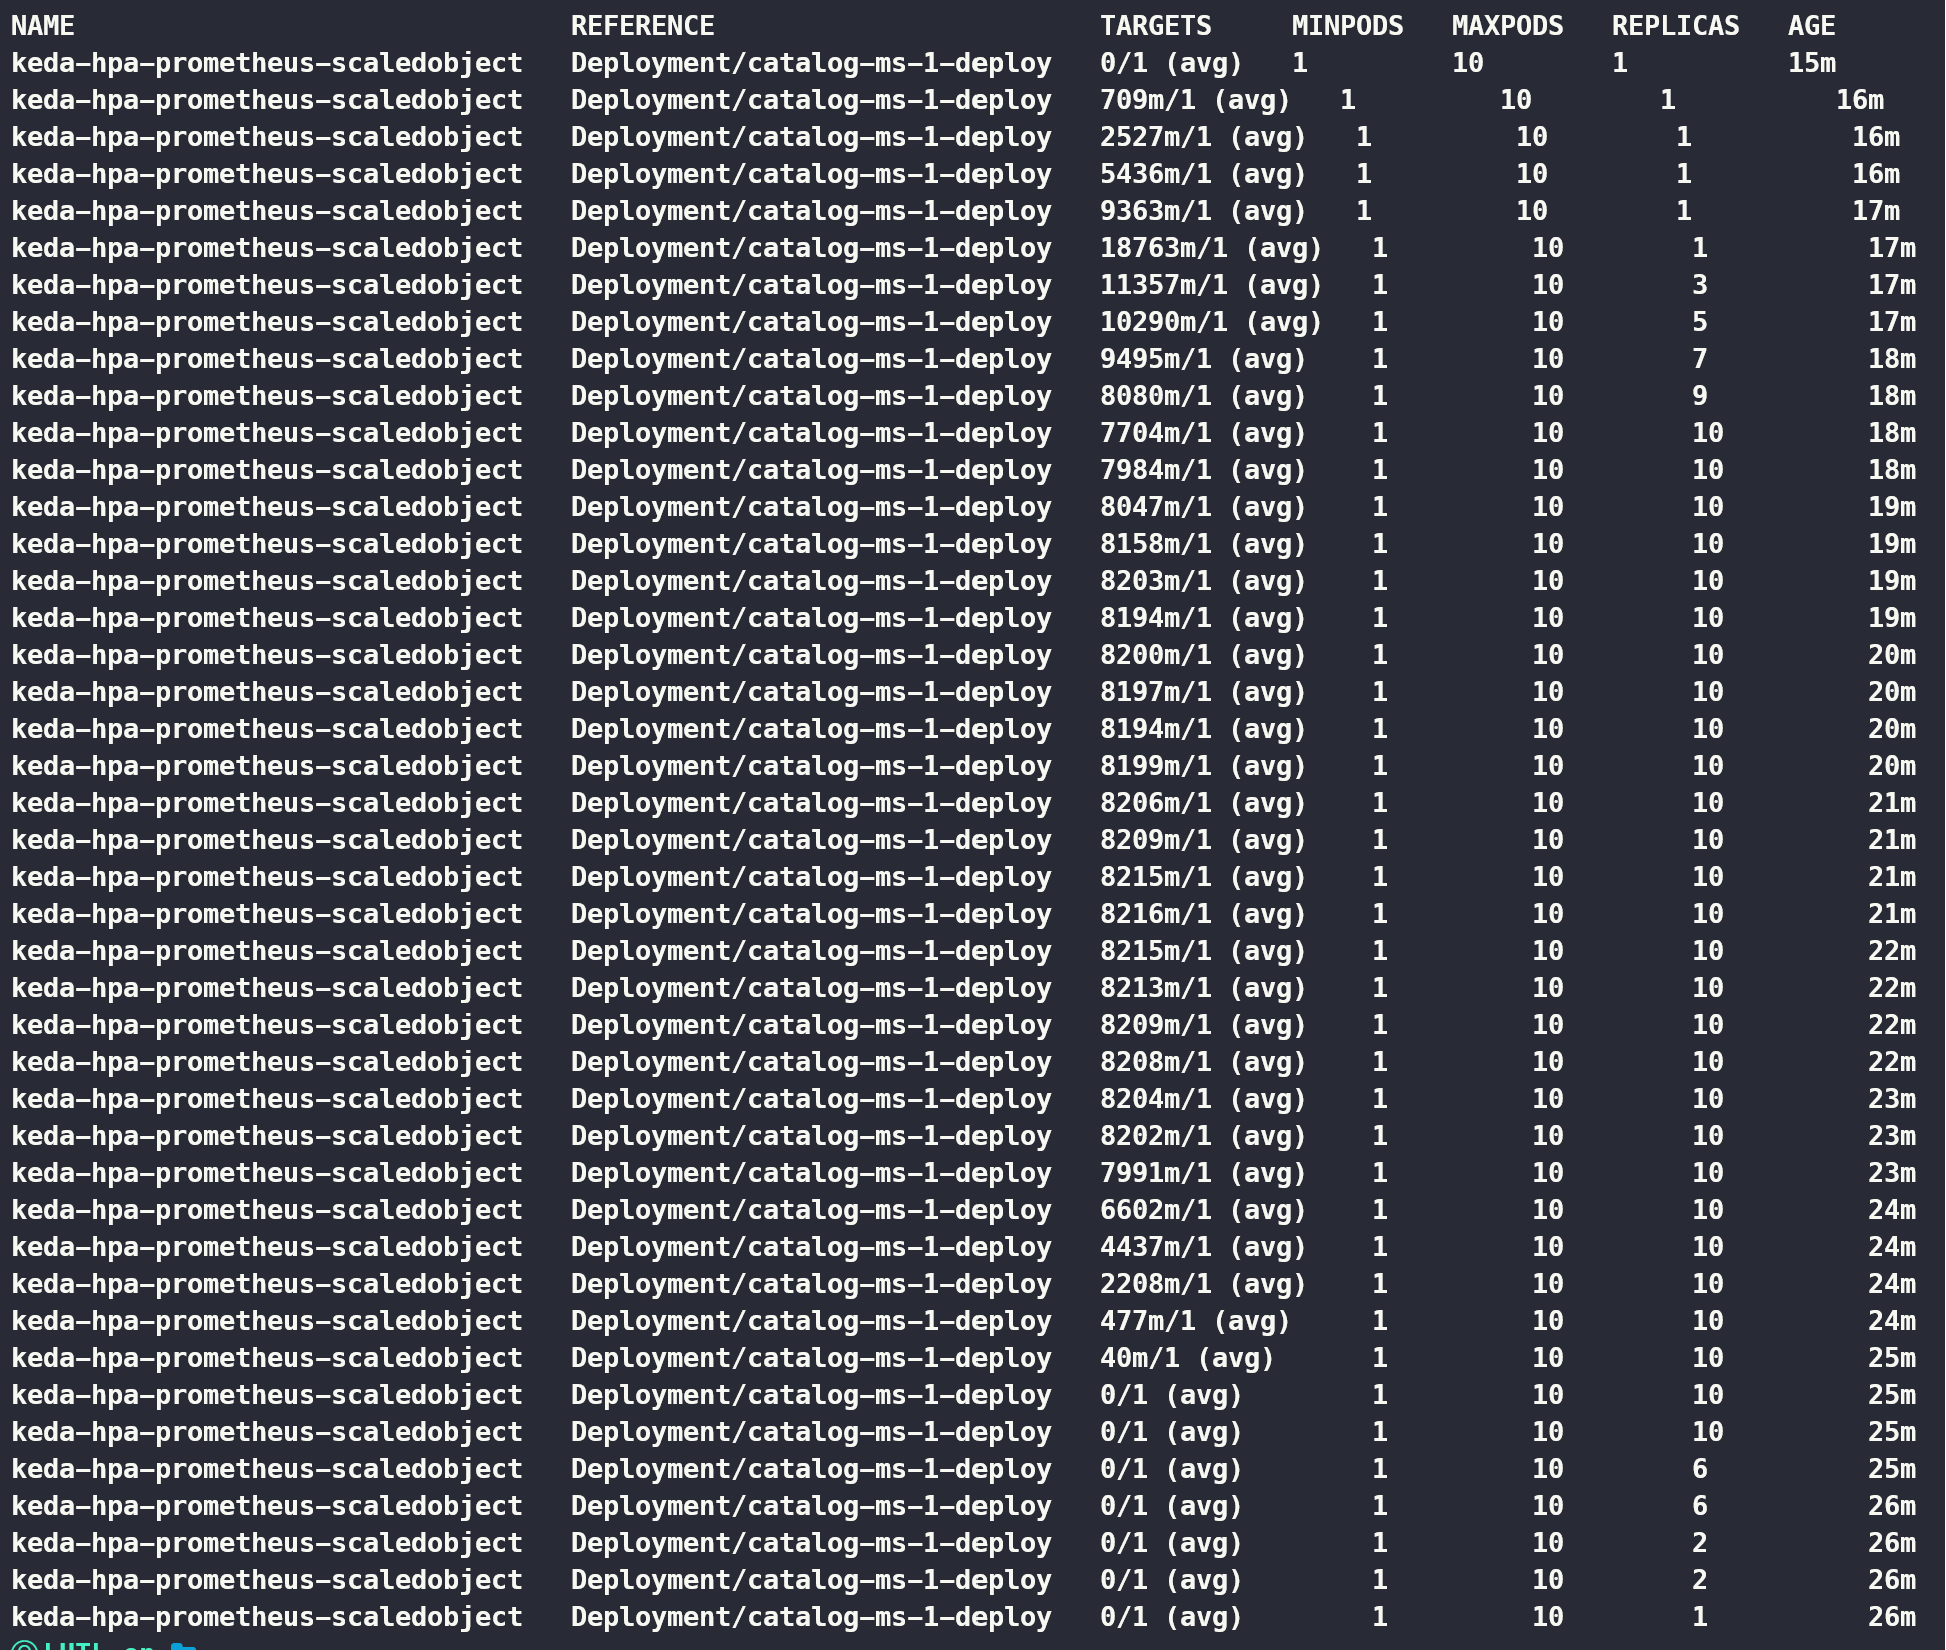
\includegraphics[scale=0.55]{images/hanh/test-with-hpa-pod-scaling.png}
    \caption{Số lượng các pod thay đổi khi chạy bài kiểm tra với k6}
  \end{center}
  \label{}
\end{figure}
Thông qua hình trên, ta dễ thấy được là ScaledObject đã làm tốt công việc của mình, khi có thể tự động scale lên số pod từ 1 lên 10 khi lượng request tăng, và khi lượng reqest giảm được một thời gian, thì đã scale xuống lại về 1.

\subsubsection{Kiểm tra tính hiệu quả của việc auto scaling thông qua số request}
\noindent Sau khi đã chắc chắn rằng ScaledObject có thể giúp ta scale số pod của microservice dựa theo lượng request, thì ta cần kiếm chứng tính hiệu quả của các thiết lập mà ta đã đưa vào hệ thống.\\[0.5cm]
Đầu tiên, ta tiến hành chạy bài kiểm tra khi dịch vụ chưa được cung cấp HPA, và kiểm tra xem dịch vụ có thể phục vụ được bao nhiêu trong tổng số request đã được gửi tới hệ thống. Ta được kết quả như hình dưới.
\begin{figure}[H]
  \begin{center}
    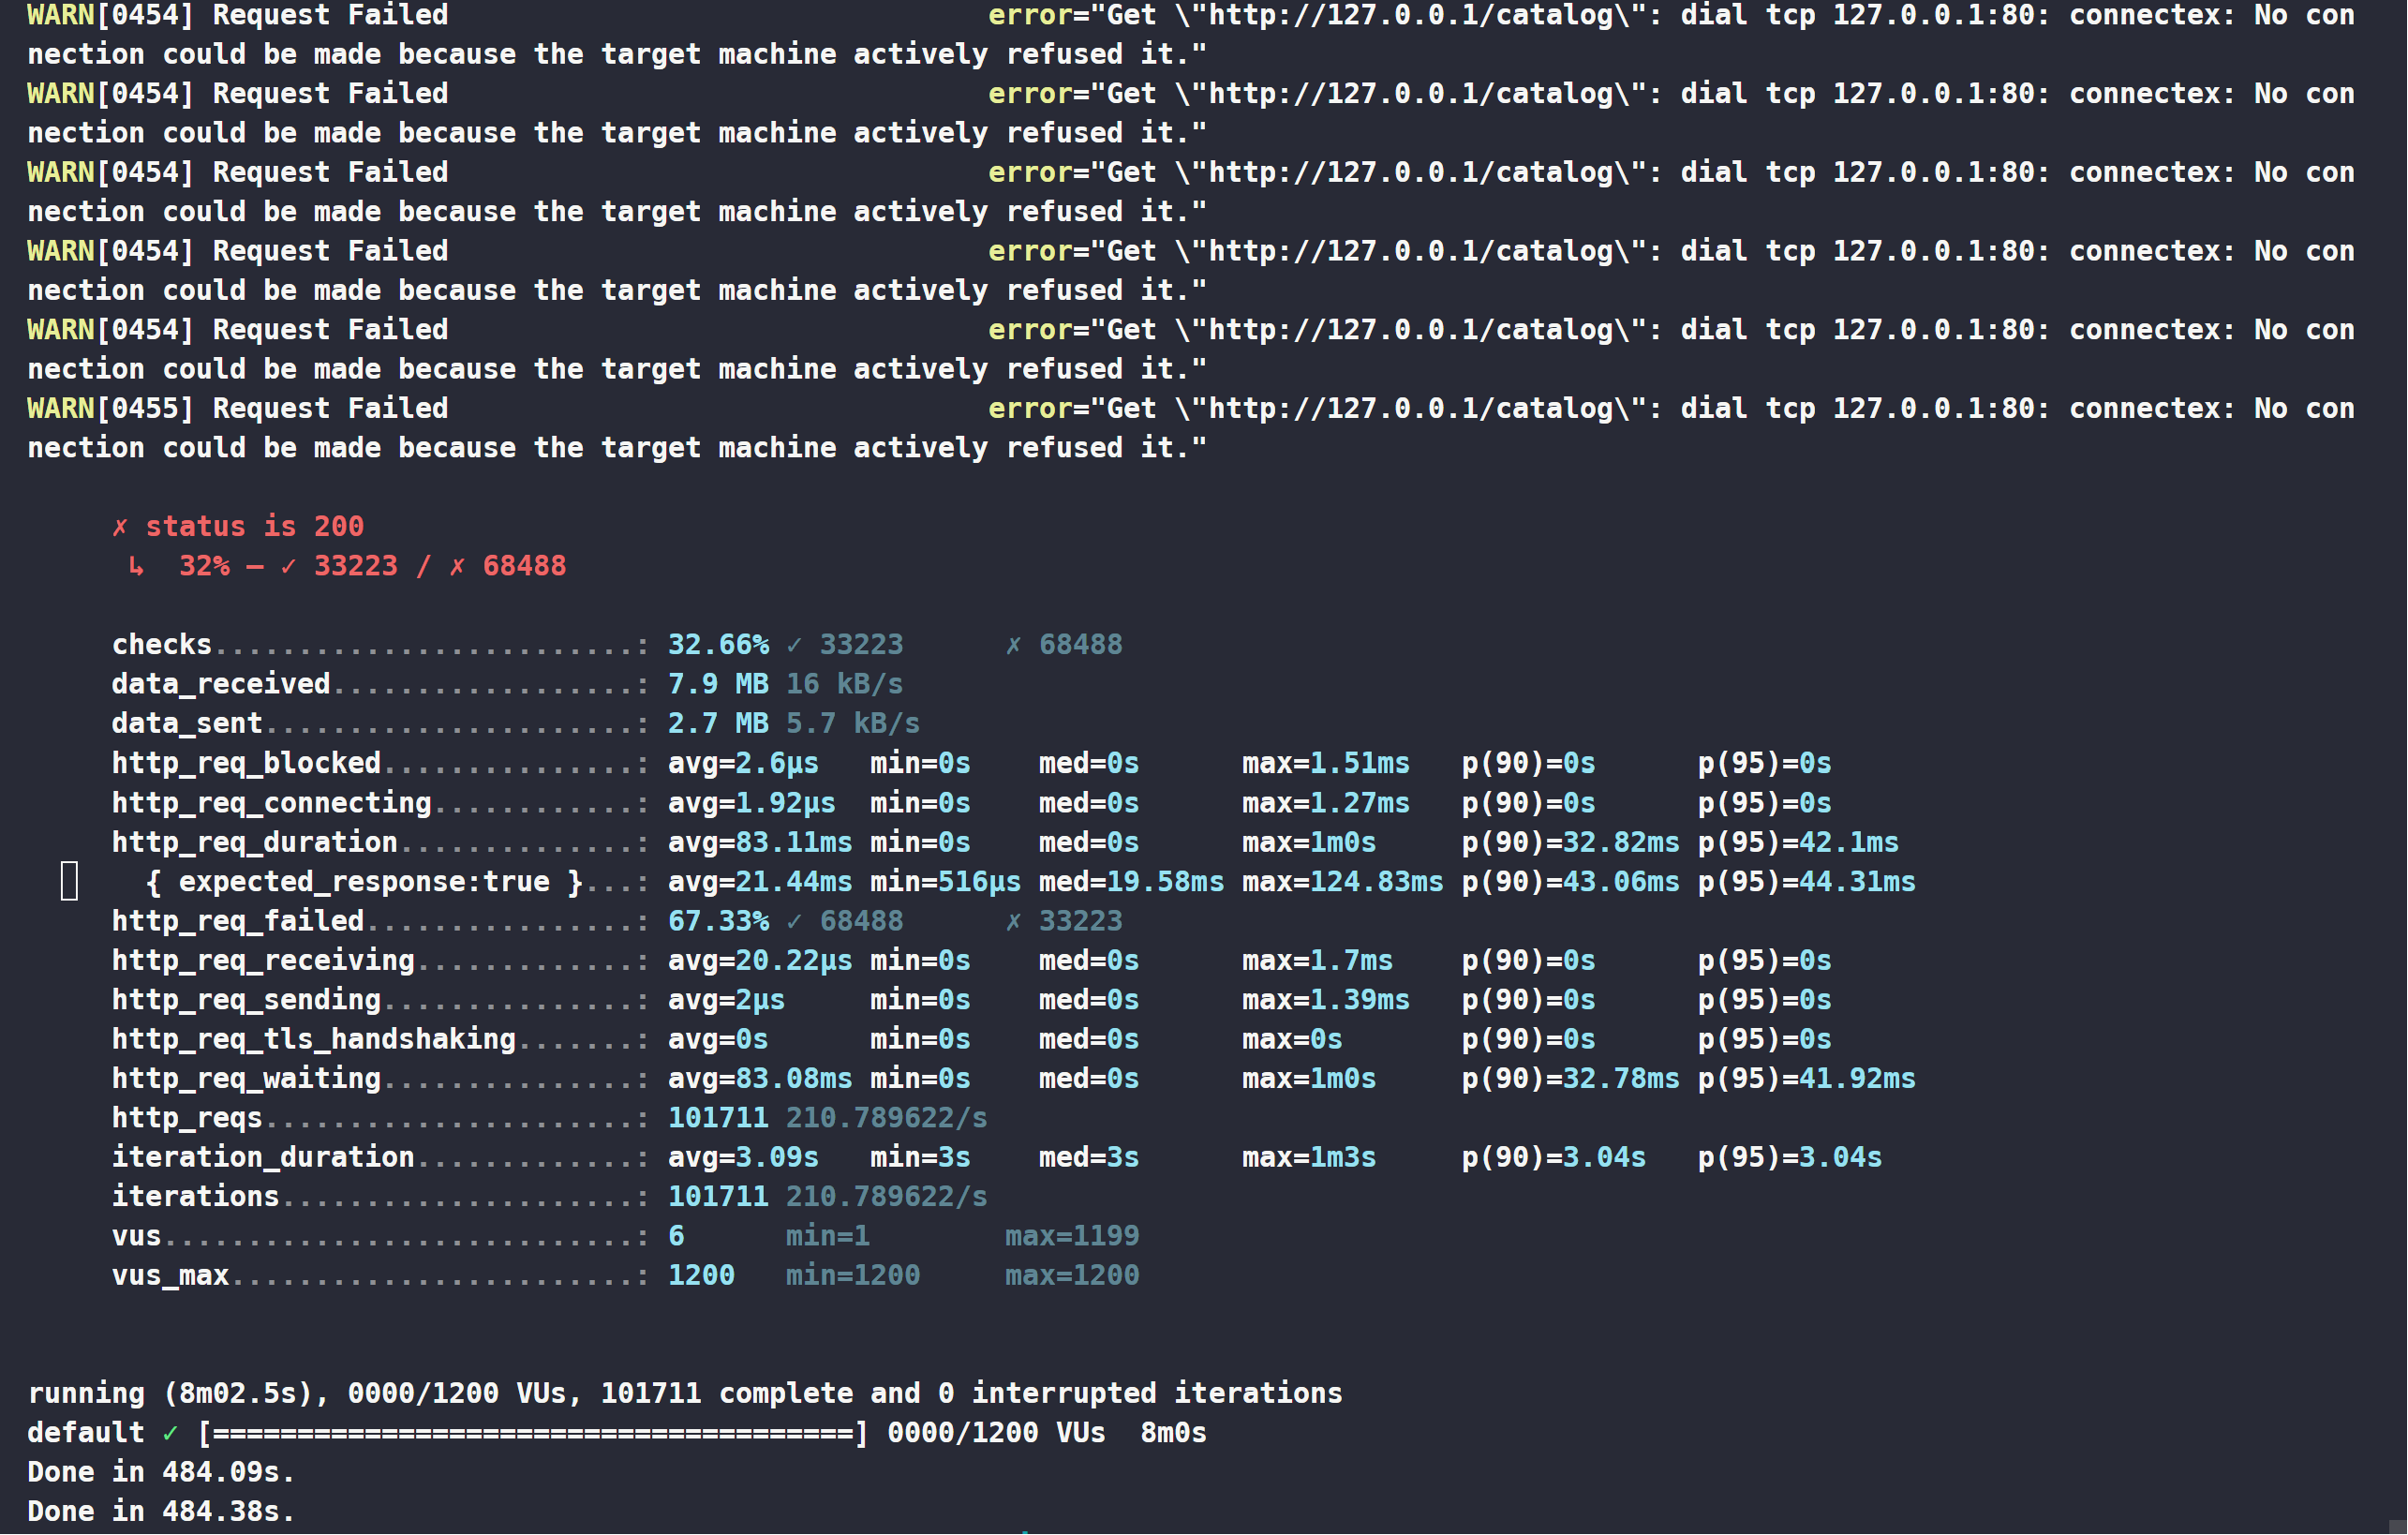
\includegraphics[scale=0.44]{images/hanh/test-without-hpa.png}
    \caption{Kết quả sau khi chạy bài kiểm tra với k6 khi dịch vụ chưa được áp dụng HPA}
  \end{center}
  \label{}
\end{figure}
Theo như hình trên, pod chỉ có thể phục vụ được 32\% số lượng request được gửi tới từ k6, một con số khá khiêm tốn. Tuy nhiên, xét việc khi cấu hình thì bản thân pod chứa Catalog microservice đã bị giới hạn tài nguyên khá nhiều, do đó điều này cũng là dễ hiểu.\\[0.5cm]
Sau đó, ta thử bài test với việc có ScaledObject, ta thu được kết quả như hình.
\begin{figure}[H]
  \begin{center}
    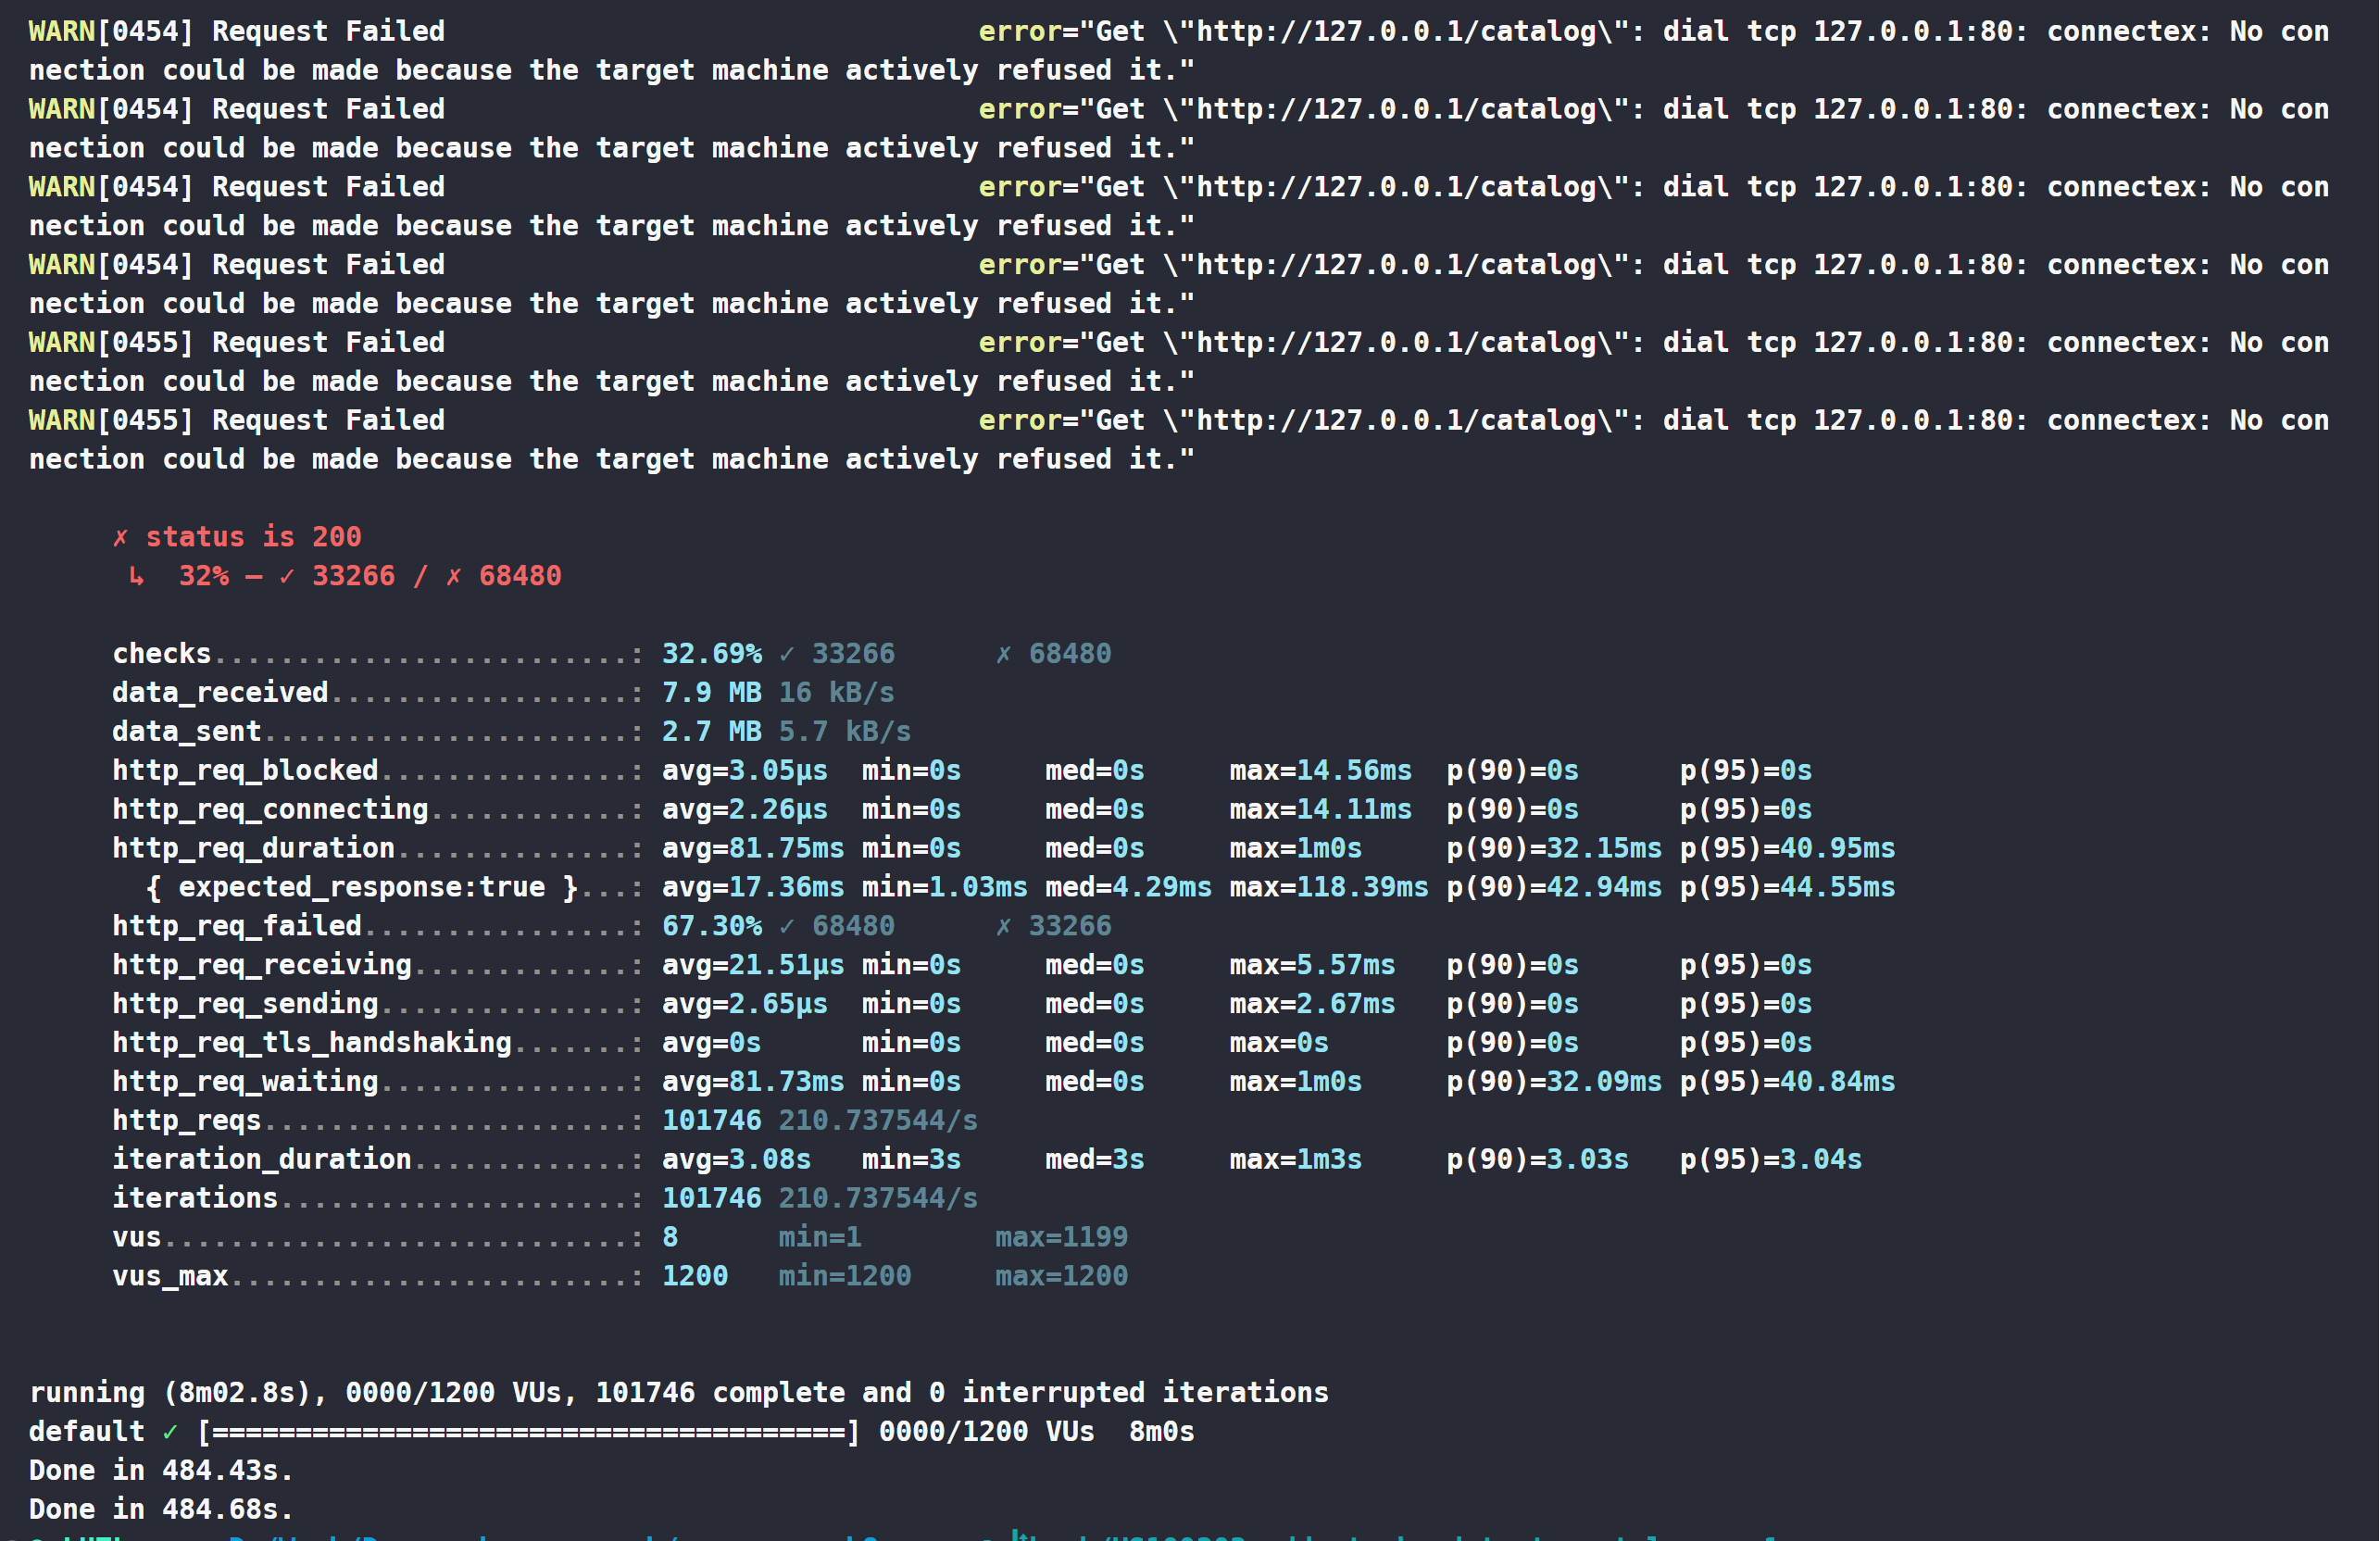
\includegraphics[scale=0.44]{images/hanh/test-with-hpa.png}
    \caption{Kết quả sau khi chạy bài kiểm tra với k6 khi dịch vụ đã được áp dụng HPA - ScaledObject}
  \end{center}
  \label{}
\end{figure}
Trong trường hợp này, việc áp dụng HPA cũng không giúp ta có thể phục vụ đươc nhiều request hơn. Theo như hình trên, ta vẫn chỉ phục vụ được 32\% số request. Vậy nguyên nhân là do đâu?\\[0.5cm]
Để tìm hiểu sâu thêm về vấn đề này, ta theo dõi hoạt động của các pod cho Catalog microservice khi bài kiểm tra đang diễn ra.
\begin{figure}[H]
  \begin{center}
    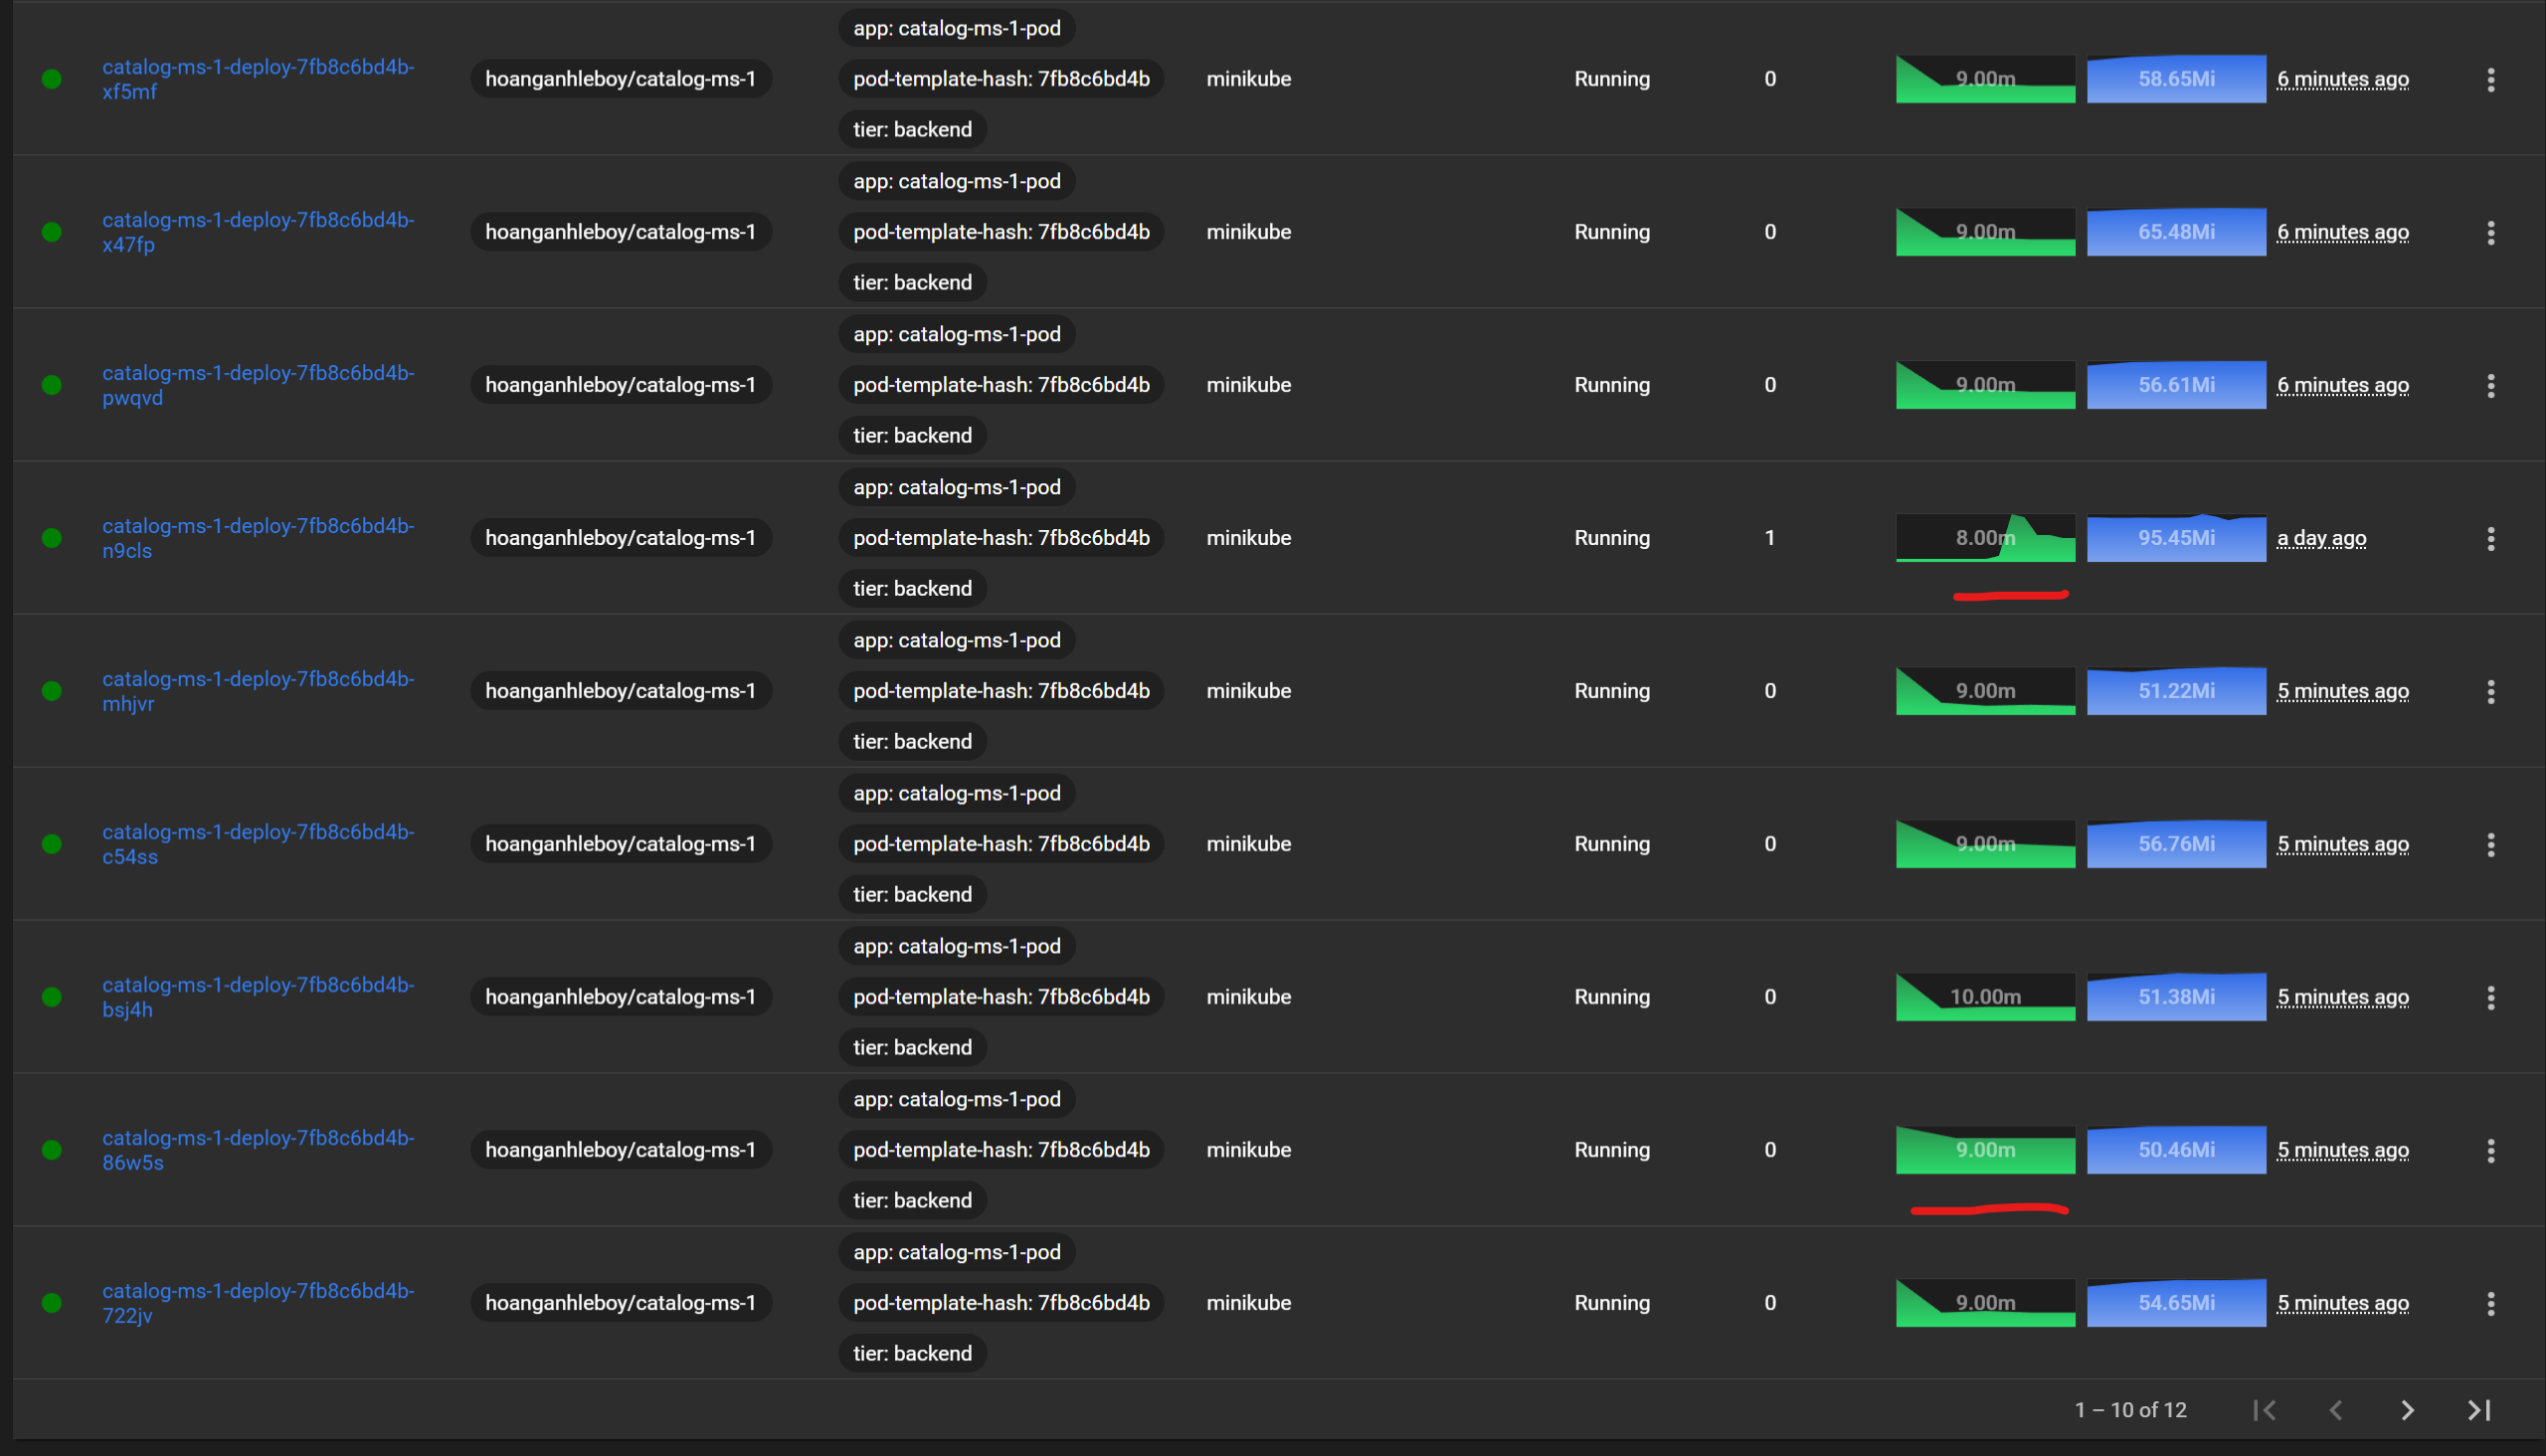
\includegraphics[scale=0.44]{images/hanh/test-with-hpa-pod-resource-ultilization.png}
    \caption{Trạng thái các pod khi diễn ra bài kiểm tra của k6}
  \end{center}
  \label{}
\end{figure}
Đi tìm hiểu sâu hơn về các chỉ số các pod của Catalog microservice, ta nhận thấy rằng chí có một vài pod (được đánh dấu đỏ trên hình), là được sử dụng gần hết công suất, thông qua việc chỉ số CPU ultilization gần tối đa. Đây là biểu hiện của việc lượng tải được phân bố không đều vào các pod, từ đó dẫn đến pod thì bị quá tải, pod thì chạy không. Nguyên nhân dẫn đến hành vi này là do môi trường giả lập Kubernetes cluster trên local không cung cấp được load balancer cho Kubernetes cluster, do đó việc chia tải từ Kubernetes service vào các bod diễn ra theo trình tự ngẫu nhiên, dẫn tới hiện tượng như miêu tả trên hình.\\[0.5cm]
\textbf{Biện pháp đề xuất:} Hiện thực cluster trên một môi trường khác có thể cung cấp được load balancer cho Kubernetes service, ví dụ như môi trường cloud.
